%Path relative to the .tex file containing the \includegraphics command
\graphicspath{ {img/} }

\chapter{Introducción}
\lhead{Capítulo 1. \emph{Introducción}}

La investigación presentada en este trabajo se centra en una problemática
existente en el paquete para optimización de la ubicación de trampas para
mosquito MGSurvE: no se cuenta con el algoritmo adecuado para generar las
posiciones óptimas de las trampas. Se propone un algoritmo como solución a
esta problemática y se evalúa su eficacia. 

\section{Motivación}

En cualquier proyecto se cuentan con recursos finitos para su desarrollo, ya
sea dinero, materiales, o en el caso de lo analizado en este trabajo, trampas
para mosquitos. Es de suma importancia lograr los mejores resultados con un
número finito de trampas para detectar las migraciones de mosquitos.

\section{Objetivo}

El principal objetivo del presente trabajo es obtener las posiciones óptimas
de trampas para mosquito y así acortar los tiempos de detección de mosquito y
lograr, en un futuro, un mejor monitoreo de variantes genéticas de interés en
una población de mosquitos dada.

\section{Estructura del trabajo}

El presente reporte está compuesto de 7 capítulos que tratan diferentes puntos
de la investigación llevada a cabo.

En el Capítulo \ref{chap:estado-del-arte}, se presenta una variedad de
términos que sirven para dar contexto de este trabajo. En seguida, se
presentan y analizan investigaciones relacionadas a la realizada en este
reporte.

En el Capítulo \ref{chap:planteaminto} se presentan las limitaciones de las
herramientas actuales y se detalla la problemática identificada.

A continuación, en el Capítulo \ref{chap:solucion}, se propone una solución
a la problemática identificada en el capítulo anterior. Se detallan todos los
componentes de la solución, desde el diseño del algoritmo hasta su
arquitectura y el tipo de parámetros necesarios para su correcto
funcionamiento.

Una vez propuesta una solución, en el Capítulo \ref{chap:metolodogia} se
detalla la metodología usada para evaluar la efectividad del algoritmo
propuesto. Se describe la búsqueda de la mejor configuración para el algoritmo
y cómo será comparado con la implementación actual del paquete MGSurvE.

En seguida, se presentan los resultados de la evaluación en el Capítulo
\ref{chap:resultados}. Se presentan una variedad de gráficas y tablas para
entender a detalle el comportamiento del algoritmo propuesto en este trabajo.

Después, se presentan en el Capítulo \ref{chap:interpretacion} las
contribuciones logradas a partir de los resultados obtenidos con la evaluación
del trabajo.

Finalmente, en el Capítulo \ref{chap:conclusiones} se presentan las
conclusiones y el posible trabajo futuro para mejorar los resultados obtenidos
por la solución propuesta.

\chapter{Estado del arte}\label{chap:estado-del-arte}
\lhead{Capítulo 2. \emph{Estado del arte}}
Antes de hablar del problema y su solución, es necesario entrar en contexto.
Por esto, en la primera sección de este capítulo se definirán conceptos
básicos, tales como trampas para mosquitos, las cuales tienen un papel central
en el problema. Enseguida, se hablará sobre términos de inteligencia
artificial y métodos de optimización, los cuales ayudarán a entender mejor las
problemática y su solución.

En la segunda parte de este capítulo se hablará de algunos trabajos recientes
para poder entender el estado del arte en problemas de optimización. Sin
embargo, por la poca investigación relacionada a la optimización de vigilancia
de mosquitos, se analizarán trabajos similares enfocados en redes y
monitoreo.

\section{Conceptos básicos}
En este trabajo se tocan temas de optimización, que es una de las ramas de la
inteligencia artificial, por lo que es conveniente definir algunos conceptos
importantes antes de continuar. 

\subsection{Inteligencia artificial}
  En el libro Artificial Intelligence: A Modern Approach
  \cite{AIModernAproach}, se define la inteligencia artificial (IA) como
  máquinas con pensamiento parecido al humano y con acciones racionales.
  
  Una definición más elaborada es la de \cite{AIDef}: IA es un término
  utilizado para etiquetar a computadoras que imitan funciones humanas
  cognitivas, tales como aprendizaje y resolución de problemas. De igual
  manera, se llama inteligencia artificial a algoritmos que trabajan con la
  misma complejidad que expertos humanos.

\subsection{Optimización}
  Puede ser definida como el proceso de encontrar la mejor solución posible
  entre todas las disponibles. Por lo tanto, la tarea de optimización es
  modelar algún problema en términos de alguna función de evaluación y emplear
  algún algoritmo de búsqueda para minimizar (o maximizar) esa función
  objetivo. Sin embargo, no es posible asegurar que el resultado óptimo será
  encontrado, ya que hay problemas demasiado grandes que es imposible
  encontrar la solución óptima \cite{SearchMethodologies}.

\subsection{Heurísticas}
  En el área computacional de optimización, se llaman heurísticas a los
  métodos usados para buscar soluciones de alta calidad, sin asegurar la
  óptima.

  Una definición más elaborada la da \cite{HeuristicDef}, pues dice
  que una técnica heurística es un método que busca soluciones buenas (y casi
  óptimas) con un costo computacional bajo. Sin embargo, estos métodos no son
  capaces de indicar qué tan cerca de la optimización perfecta se encuentra 
  la respuesta actual dada por una heurística.

\subsection{Metaheurísticas}
  Se refiere a técnicas que coordinan, manipulan y guían el comportamiento y
  soluciones de métodos heurísticos de optimización. Tales métodos pueden ser
  desde procedimientos de alto nivel o pueden describir las alteraciones
  posibles para una heurística \cite{MetaheuristicsDef}.

  Existe una gran cantidad de metaheurísticas
  \cite{HeuristicDef, SearchMethodologies}, más adelante se hablará de algunos
  métodos, tal como algoritmos genéticos y optimización de enjambre de
  partículas.

\subsection{Inteligencia de enjambre}
  La inteligencia de enjambre es un campo computacional que diseña y estudia
  algoritmos para buscar soluciones a problemas. Estos algoritmos están 
  inspirados en el comportamiento complejo y, algunas veces, coordinado de
  enjambres de cualquier organismo natural \cite{SearchMethodologies}. 
  
  \begin{figure}[ht!]
    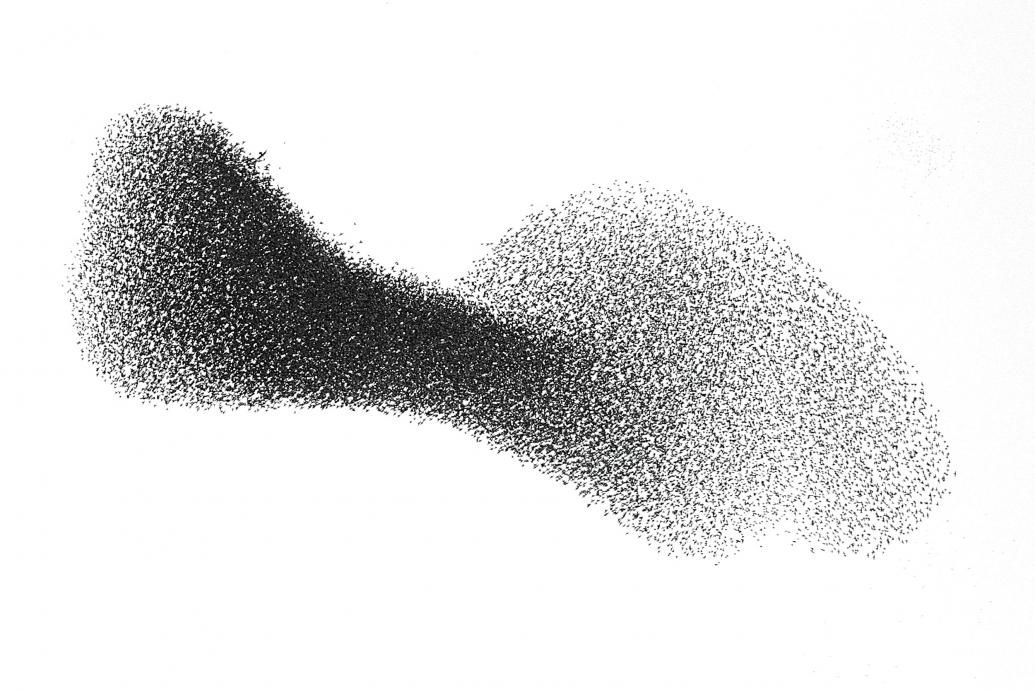
\includegraphics[scale=0.18]{si-repr}
    \centering
    \caption{Inspiración de algoritmos de inteligencia de enjambre.}
    \centering
  \end{figure}

\subsection{Algoritmos evolutivos}
  Son un tipo de algoritmos que buscan soluciones a problemas, tomando
  inspiración de la selección natural y genética \cite{EADef,GADef}. Estos 
  algoritmos pueden representar cromosomas como cadenas de texto, los cuales 
  son las soluciones a los problemas; los alfabetos representan genes; y más
  conceptos tomados de la biología.

\subsection{Particle Swarm Optimization}\label{subsec:pso}
  Particle Swarm Optimization (PSO) fue inventada por Eberhart y Kennedy en
  1995 \cite{PSODef}, es un algoritmo
  estocástico inspirado en el comportamiento de una parvada de aves en busca
  de alimento. Cada partícula en el algoritmo, que representa una solución al
  problema, vuela en el espacio de búsqueda, actualizando su velocidad y su
  posición. La ecuación clásica para actualizar la velocidad de una partícula
  es \ref{eq:1} y para actualizar su posición es \ref{eq:2}.

  \begin{equation}
    \label{eq:1}
    v_{ij} = v_{ij} + c_1 rand()(p_{ij} - x_{ij}) + c_2 rand()(p_{nj} - x_{ij})
  \end{equation}

  \begin{equation}
    \label{eq:2}
    x_{ij} = x_{ij} + v_{ij}
  \end{equation}

  Actualmente, el algoritmo PSO canónico (CPSO) o PSO con peso inercial
  (PSO-iw) es considerado como el PSO estándar \cite{CPSO,PSOReview}.
  En esta forma de PSO, se introduce una nueva variable $w$, modificando
  \ref{eq:1} a \ref{eq:3}. Esta nueva variable equilibra la búsqueda local y
  global de la solución.

  \begin{equation}
    \label{eq:3}
    v_{ij} = w v_{ij} + c_1 rand()(p_{ij} - x_{ij}) + c_2 rand()(p_{nj} - x_{ij})
  \end{equation}

\section{Trabajos relevantes en el área}
En esta sección, después de haber definido conceptos importantes, se
detallarán y analizarán algunos trabajos relevantes en el área que describen
el estado del arte en optimización de posicionamiento de nodos en diferentes
tipos de redes.

\subsection{Optimización de ubicación de una red de sensores inalámbricos en
  un taller inteligente}
  En el primer trabajo de esta sección, de 2018, Li et al \cite{3DAFAO}
  desarrollaron un nuevo algoritmo con el
  objetivo de optimizar la ubicación de nodos de una red de sensores
  inalámbricos (WSN) para minimizar el error de detección de objetos 3D en un
  taller de manufactura inteligente.
  
  Los autores tomaron inspiración del comportamiento de enjambres de moscas,
  e implementaron en algoritmo de 
  optimización de moscas (FOA). Sin embargo, este algoritmo presenta un
  comportamiento 2D, y su problema necesita un análisis en tres dimensiones.
  Por esto, introdujeron una nueva dimensión en la búsqueda de soluciones,
  resultando en el algoritmo es 3D-FOA. Como una alternativa, decidieron
  añadir una variable más a su algoritmo, un peso inercial variable,
  proveniente de PSO-iw, resultando en un nuevo algoritmo: 3D-AFOA.

  Al tener dos algoritmos capaces de optimizar los nodos de la red MSN,
  realizaron diversos experimentos para comparar dichos métodos. Inicialmente,
  establecieron la posición fija de 3 nodos de la red y un solo nodo objetivo
  a detectar en un taller simulado. Establecieron una población de 50 y 500
  como número máximo de generaciones en ambos algoritmos. En la figura
  \ref{fig:location-error-3d-foa-3d-afoa_1} se muestran los resultados
  obtenidos.

  \begin{figure}[ht!]
    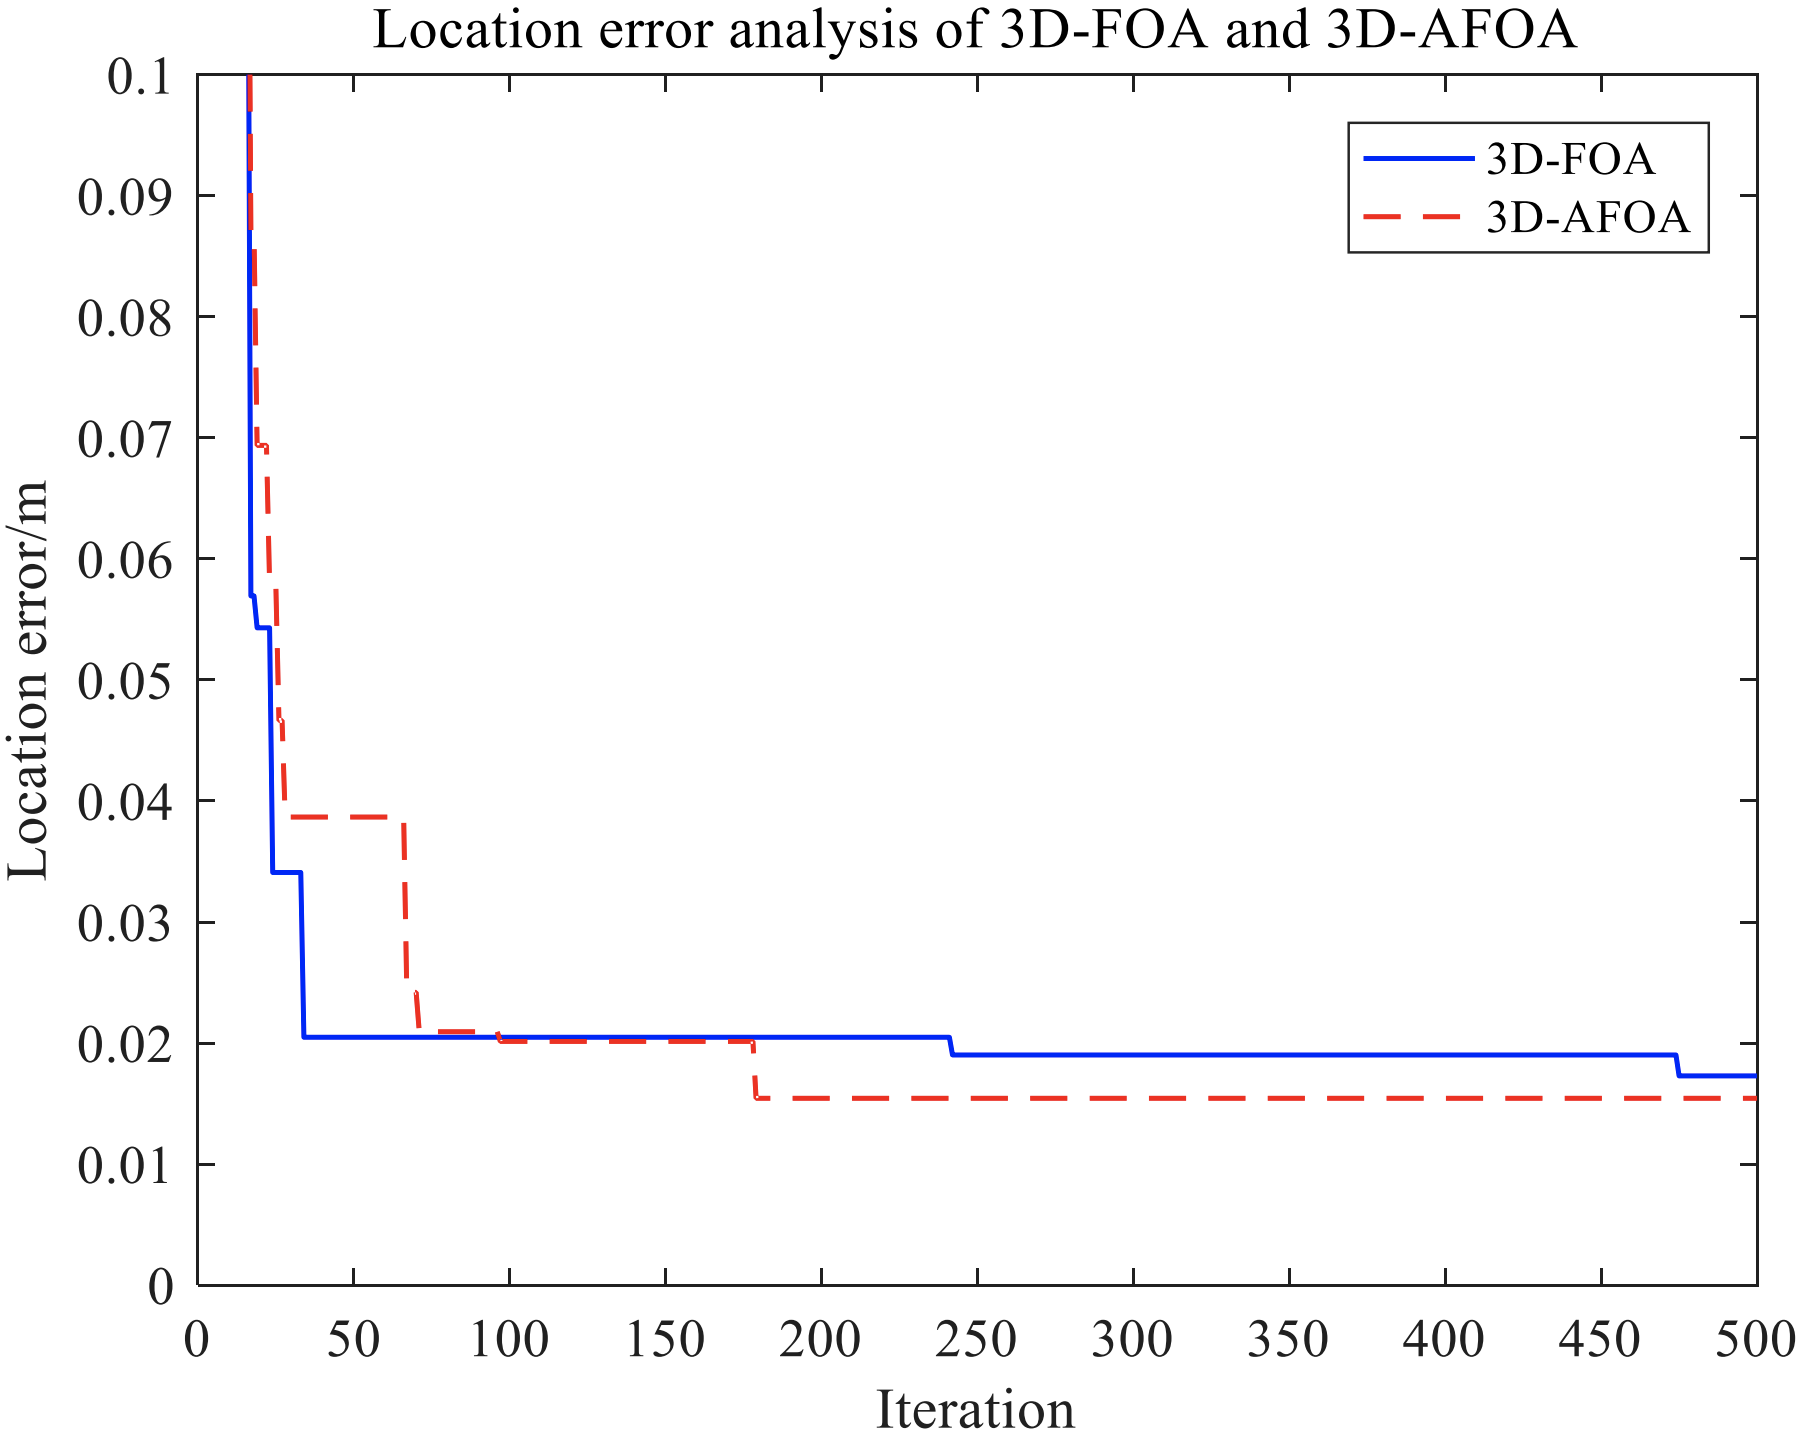
\includegraphics[width=\textwidth]{location-error-3d-foa-3d-afoa_1.png}
    \centering
    \caption{Resultados de error de detección de 3D-FOA y 3D-AFOA.}
    \label{fig:location-error-3d-foa-3d-afoa_1}
    \centering
  \end{figure}

  Como se puede ver en la figura \ref{fig:location-error-3d-foa-3d-afoa_1}, el
  algoritmo 3D-AFOA tiene un mejor desempeño, pues converge en una mejor
  solución en menos generaciones. 

  Cone l objetivo de verificar la efectividad del algoritmo, se probó con 3, 4
  y 5 nodos fijos en la red para detectar nuevamente un recurso en el taller
  simulado. Los resultados se muestran en \ref{fig:location-error-3d-afoa_2}.

  \begin{figure}[ht!]
    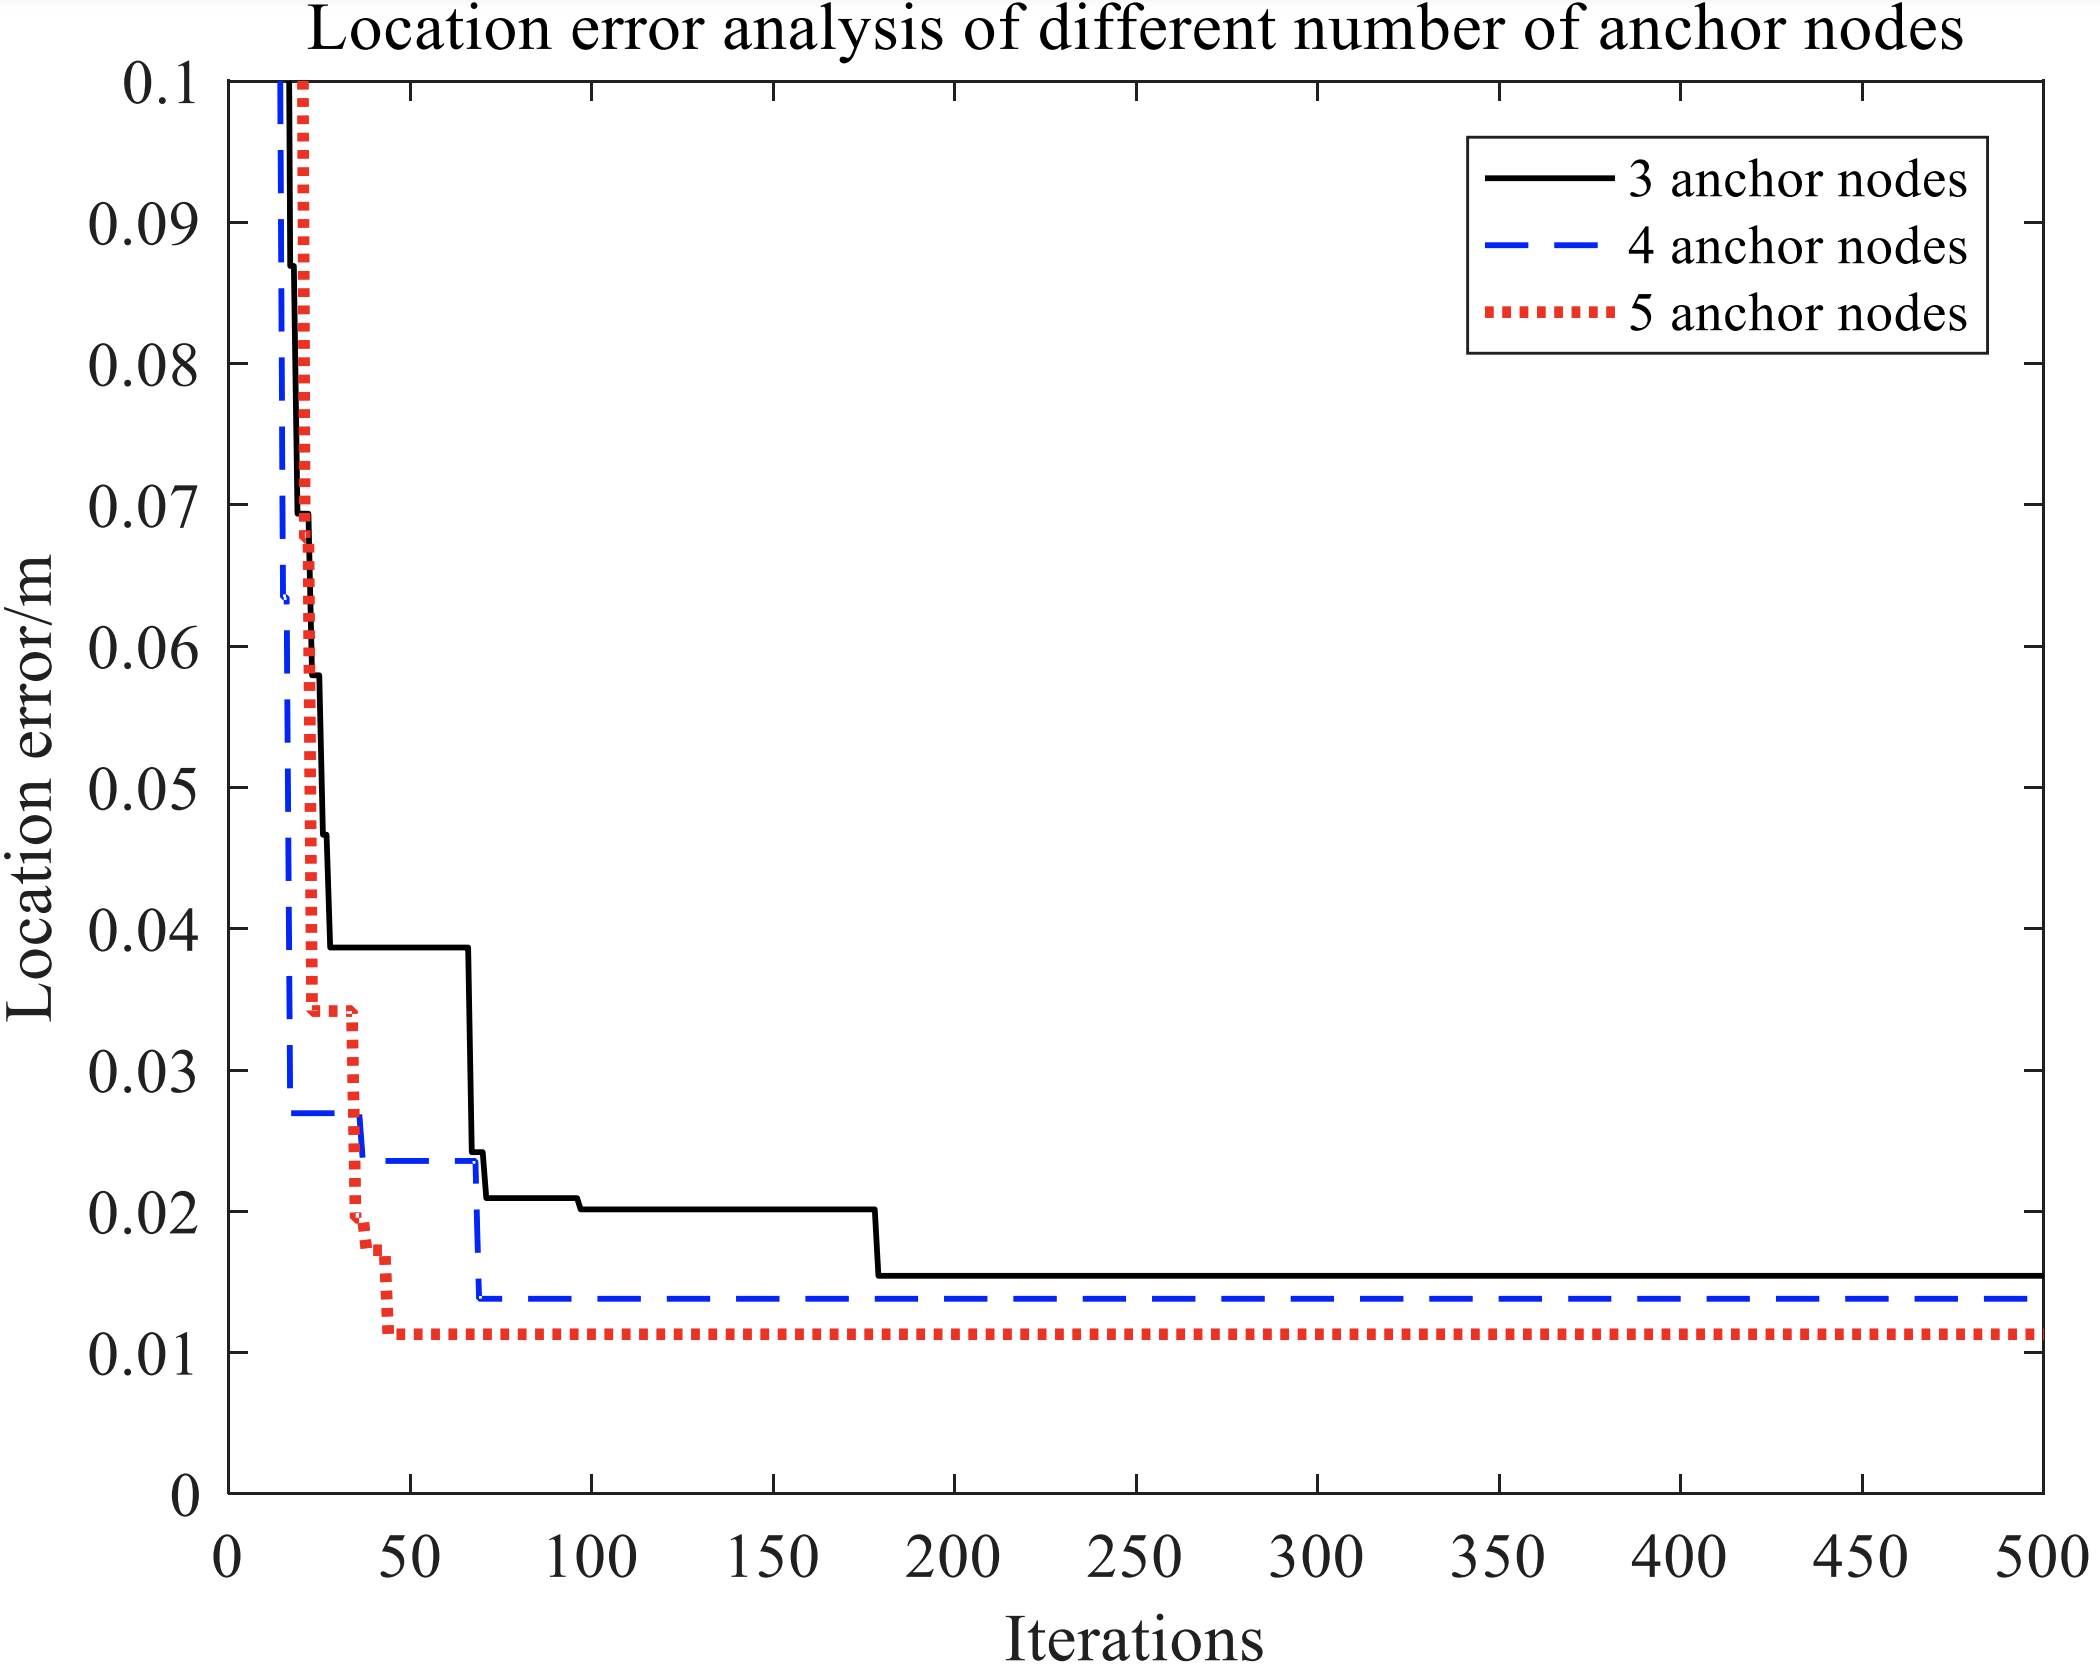
\includegraphics[width=\textwidth]{location-error-3d-afoa_2.png}
    \centering
    \caption{Resultados de error de detección con diferente cantidad de
      nodos.}
    \label{fig:location-error-3d-afoa_2}
    \centering
  \end{figure}

  Analizando los resultados expuestos en \ref{fig:location-error-3d-afoa_2},
  se puede apreciar que, conforme incrementa el número de nodos en el
  algoritmo, el tiempo de convergencia acelera. Sin embargo, el
  error de detección de los objetivos, aunque mejora con más nodos, no existe
  gran diferencia. Esto es debido a que solamente la ubicación de un solo nodo
  fue optimizada en los algoritmos. 

  Para finalizar, los investigadores concluyeron que 3D-AFOA es altamente
  aplicable al problema de optimización en la ubicación de nodos en una red
  WSN y no requiere de un alto presupuesto computacional para lograr buenas
  soluciones. 

\subsection{Asignación óptima de unidades de generación distribuidas en
  sistemas de energía radiales}
  Como segundo trabajo relevante presentado en esta sección, Hantash et al,
  en 2020 \cite{PSOEnergy}, publicaron un estudio en el que
  proponen una modificación al estándar PSO-iw para calcular las posiciones y
  tamaños de unidades generadoras distribuidas en una red radial de energía
  eléctrica. 

  Los autores partieron del estándar PSO-iw y, después de una investigación,
  encontraron que valores grandes en el peso inercial ($w$) facilitan la
  búsqueda global, mientras que valores pequeños de $w$ favorecen la búsqueda
  local \cite{CPSO, APSO2016}. Gracias a estos hallazgos, los autores proponen
  una estrategia no
  lineal para obtener valores de $w$ variables con el tiempo. Esta estrategia
  está descrita en la Ecuación \ref{eq:4}:

  \begin{equation}
    \label{eq:4}
    w = w_{max} e^{(((maxiter - iter) / maxiter) - 1)} - w_{min} 
  \end{equation}
  en donde $w_{max}$ es el peso máximo, $w_{min}$ es el peso mínimo, $iter$ es
  la iteración actual y $maxiter$ es el número máximo de iteraciones.

  Finalmente, para validar sus resultados, el grupo de investigadores
  decidió comparar su
  estrategia propuesta contra un PSO convencional. Para comparar los
  resultados arrojados por ambos algoritmos, se usó la red de energía estándar
  IEEE 34. Después de la ejecución de los experimentos, los investigadores
  obtuvieron pérdidas de energía 31.6\% menores con su propuesta de PSO a
  comparación del PSO convencional sin el valor de $w$ variable. Además de
  esto, la propuesta consumió 62.2325 s para proveer una solución optima,
  cuando el PSO convencional consumió 62.2325 s. La comparación completa
  entre el PSO propuesto y el convencional está en la Figura
  \ref{fig:pso-iw-variable-comp}.

  \begin{figure}[ht!]
    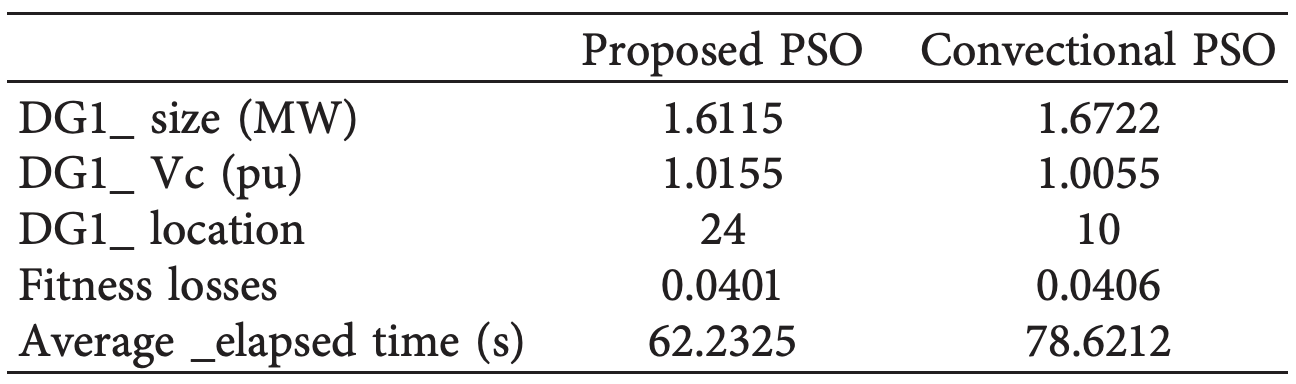
\includegraphics[width=\textwidth]{pso-iw-variable-comp.png}
    \centering
    \caption{Comparación de resultados entre el PSO propuesto y el
      convencional.}
    \label{fig:pso-iw-variable-comp}
    \centering
  \end{figure}

\subsection{Optimización de ubicación de trampas para mosquitos}
  \label{subsection:mgsurve}
  Para finalizar esta sección, se describe el
  trabajo realizado por Sánchez y el Departamento de bioestadística y
  epidemiología de la universidad de Berkley \cite{MGSurvE} que aún no ha sido
  publicado y sigue en progreso, sin embargo, es el estado del arte en el área
  de este trabajo. Sánchez et al están trabajando en un paquete llamado
  MGSurvE, el cual está diseñado para optimizar la ubicación de trampas de
  mosquito en entornos espacialmente heterogéneos. 

  En el estado actual del paquete cuenta con diversas funcionalidades, tales
  como: diferentes kernels de movimiento para mosquitos machos y hembras;
  kernels de atractivo para trampas personalizables; soporte para trampas
  inamovibles; rutinas de trazado de mapas integradas; integración de rutinas
  para optimización con GA; y mucho más, con más funciones esperadas en
  futuras actualizaciones.

  Como se mencionó, las rutinas de optimización para la ubicación de las
  trampas para mosquito se implementa un algoritmo genético (GA), el cual es
  la variante estándar y es importado directamente del paquete DEAP
  \cite{DEAP}.

  Para el correcto funcionamiento del algoritmo de optimización, 3 grupos de
  características deben ser definidas: del entorno, de las trampas y del
  comportamiento de migración de mosquitos. En la figura
  \ref{fig:mgsurve-landscape-diagram} se describe cómo estos tres grupos de
  características forman el "Landscape", el cual es usado por el algoritmo 
  genético. 

  \begin{figure}[ht!]
    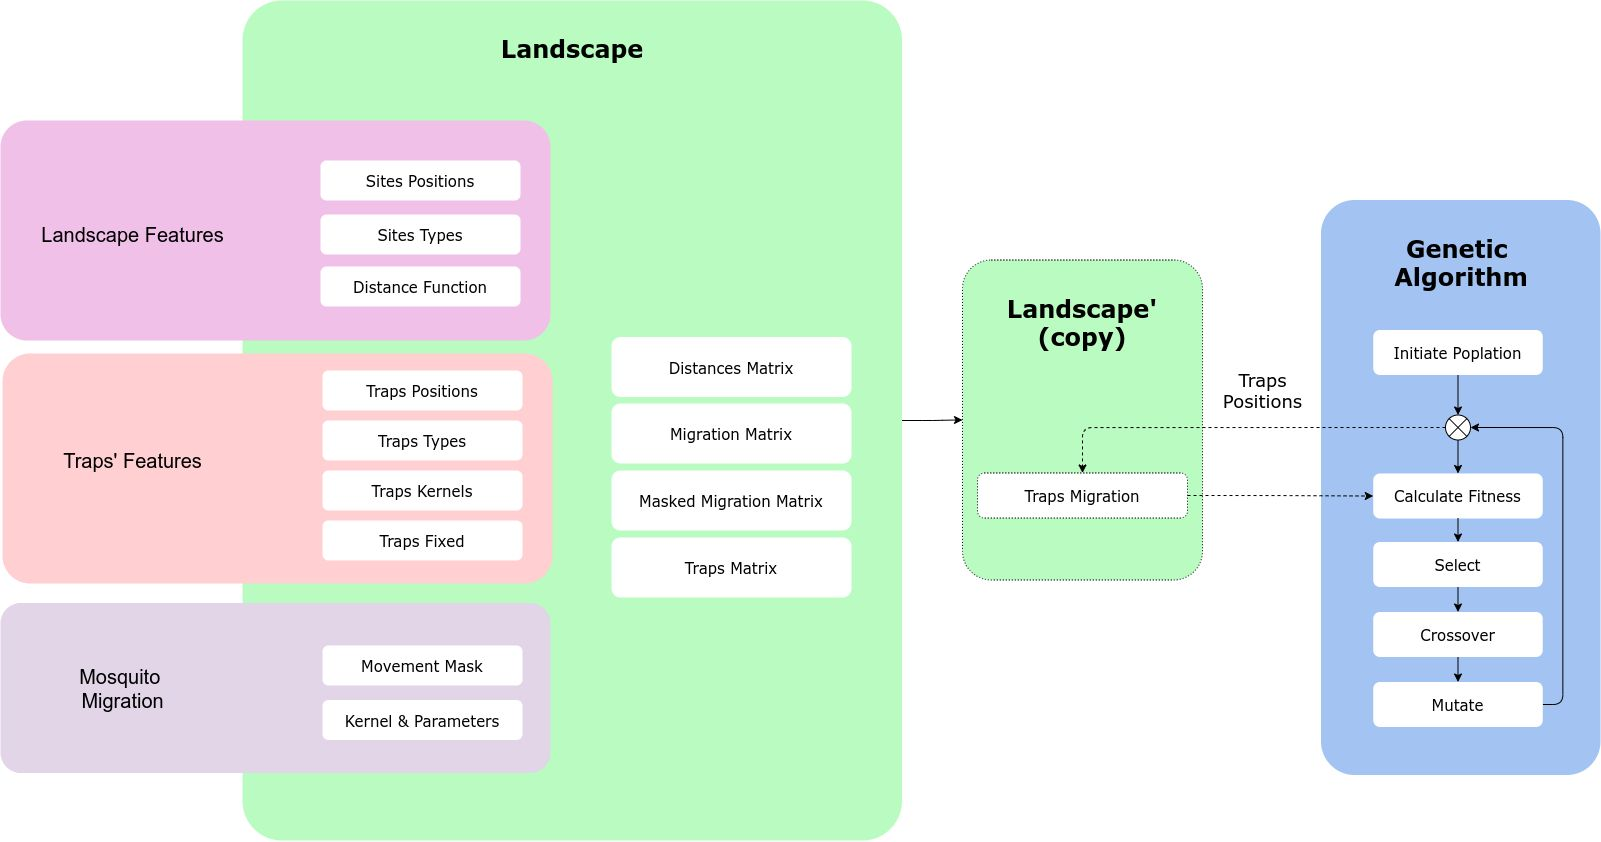
\includegraphics[width=\textwidth]{fig:mgsurve-landscape-diagram.jpeg}
    \centering
    \caption{Interacción del Landscape con el algoritmo genético.}
    \label{fig:mgsurve-landscape-diagram}
    \centering
  \end{figure}

  En la fecha de realización de este capítulo, aunque no hay ningún
  experimento publicado oficialmente, la documentación del paquete sí cuenta
  con ejemplos y tutoriales de optimización en la siguiente URL
  \url{https://chipdelmal.github.io/MGSurvE/build/html/GA.html}. En los
  tutoriales, el número de población es de 10 por cada trampa a optimizar. Si
  se desean optimizar 4 trampas, se utiliza una población de entre 40 o 50.
  Además de definir la población, también se limita a 500 generaciones para
  la optimización.

  Para finalizar, el paquete permite obtener el mejor cromosoma y trazar en un
  diagrama el mapa de las trampas y la migración de los mosquitos.

\section{Comparación de algoritmos}
\label{section:analisis}
Los trabajos mencionados en la sección anterior proponen diferentes algoritmos
para solucionar problemas muy similares: encontrar la mejor ubicación de nodos
en una red de nodos para optimizar algún resultado de una medición. Un aspecto
en común de las soluciones propuestas por los diferentes investigadores es que
todos hacen uso de algoritmos metaheurísticos iterativos para optimización.
Otra similitud es que sus soluciones están basadas en inteligencia de enjambre
y más específicamente en PSO. 

Para resaltar las ventajas y desventajas de los diferentes tipos de
algoritmos, en la tabla \ref{table:pso-ga-pros-cons} se muestra una
comparación detallada entre PSO y GA.

\begin{figure}[ht!]
  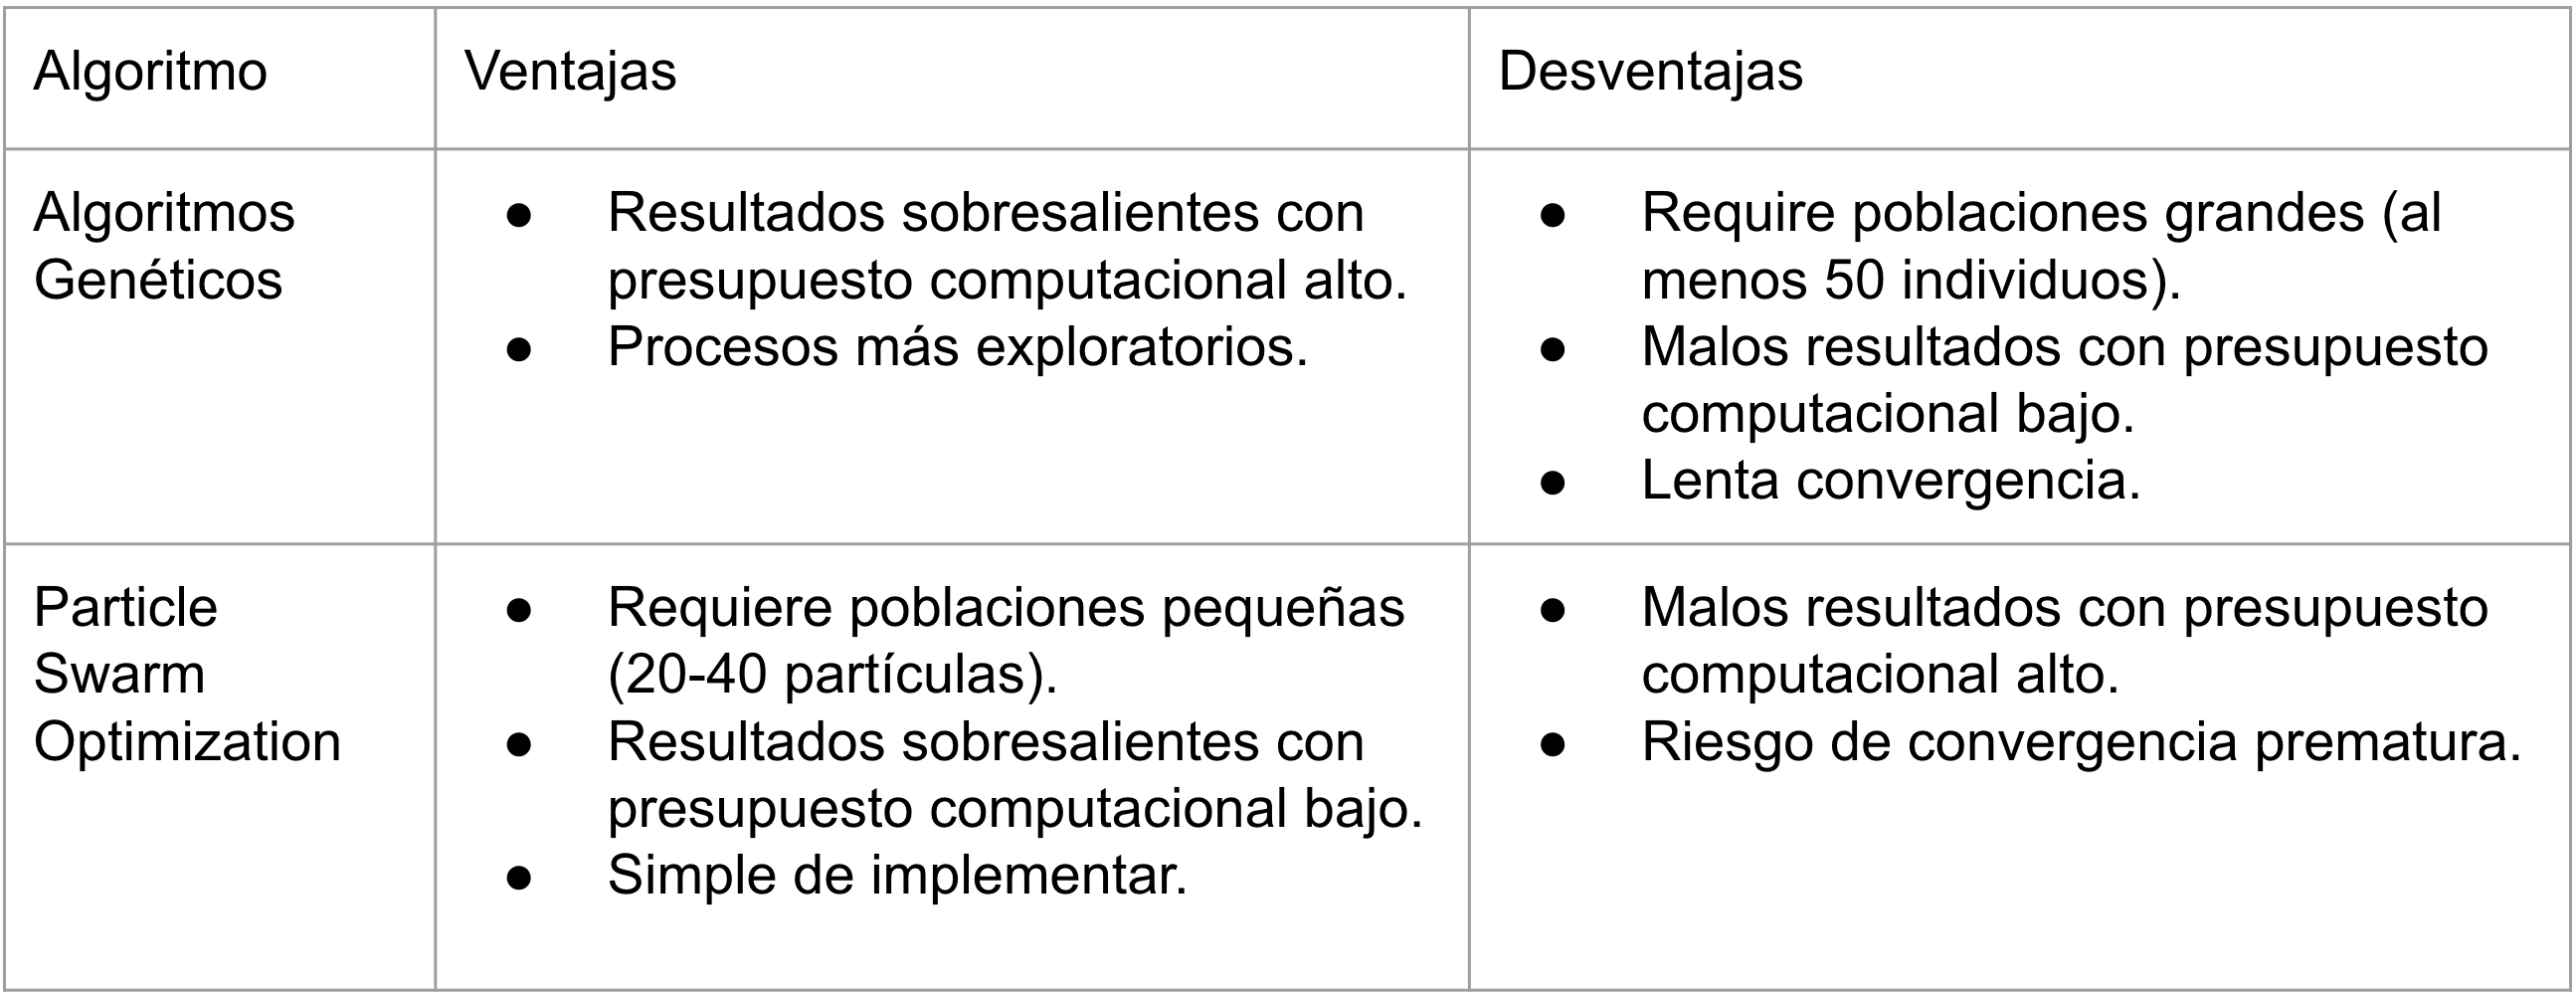
\includegraphics[width=\textwidth]{pso-ga-pros-cons.png}
  \caption{Ventajas y desventajas de PSO y GA basado en
    \cite{DE&PSOCov, SwarmVsEvol}.}
  \label{table:pso-ga-pros-cons}
\end{figure}

Además de los algoritmos propuestos por las investigaciones mencionadas en la 
sección anterior, se pueden encontrar una gran variedad usados en la
actualidad para 
resolver problemas optimización. En un estudio realizado en 2021 por
Piotrowski et al \cite{DE&PSOCov}, encontraron que las principales familias de
algoritmos usados para resolver problemas de optimización relacionados a la 
pandemia de COVID-19 fueron Swarm Intelligence (SI) y Evolutionary Algorithms
(EA). 

En 2017, un estudio similar realizado por Piotrowski et al \cite{SwarmVsEvol},
sometieron a 33 metaheurísticas propuestas entre 1960 y 2016 a 22
experimentos, cada una con diferentes presupuestos computacionales.
Al finalizar los experimentos, encontraron que algoritmos basados en
inteligencia de enjambre tienen un mejor desempeño cuando el presupuesto
computacional es bajo. A diferencia de los algoritmos basados en inteligencia
de enjambre, los basados en procesos evolutivos tienen un mejor desempeño
cuando el presupuesto computacional es alto. 

Aunque lo anterior es cierto, en un estudio de 2020 realizado por Piotrowski
et al \cite{PSOPopulationSize}, se encontró que variantes modernas de PSO y
SI sin peso inercial
logran mejores resultados con una población de entre 70 y 500 partículas,
contradiciendo las recomendaciones para lograr mejores resultados con
variantes clásicas.
Debido a esto, es de gran importancia conocer las condiciones adecuadas para
cada variante de algoritmos basados en PSO. Si la cantidad adecuada de
partículas para un problema en cuestión es desconocido, la recomendación es
usar entre 70 y 100 partículas.

\section{Conclusión}
En la actualidad, existe una gran variedad de algoritmos de optimización los
cuales tienen comportamientos diferentes para cada tipo de problema
\cite{SwarmVsEvol}. Por esto, es de suma importancia escoger correctamente el
algoritmo que será empleado en alguna solución, para así obtener resultados
realmente óptimos.

Como se ve en la tabla \ref{table:pso-ga-pros-cons} y se discutió en la
sección anterior, los algoritmos genéticos tienen un mejor comportamiento y
desempeño cuando el presupuesto computacional y la población es grande
(más de 50), por lo que el trabajo realizado en MGSurvE \cite{MGSurvE} no
está optimizando correctamente las ubicaciones de las trampas para mosquitos,
pues usan poblaciones de entre 40 y 50, además de un presupuesto computacional
bajo. Esta situación da paso a una oportunidad de mejora, para implementar un
algoritmo que se ajuste en mejor manera a la situación de MGSurvE, con la
posibilidad de mejorar la optimización de la ubicación de las trampas para
mosquitos.

\chapter{Planteamiento del problema}\label{chap:planteaminto}
\lhead{Capítulo 3. \emph{Planteamiento del problema}}
Después de analizar diferentes métodos de optimización aplicados en el área de
este trabajo, el objetivo de este capítulo es describir la problemática en
la optimización de la ubicación de trampas para mosquito. Para lograrlo, en
este 
capítulo primeramente se dará un poco de contexto sobre la herramienta actual,
enseguida se hablará sobre problemas y limitaciones con la herramienta actual
y finalmente se concluirá con el planteamiento del problema.

\section{Contexto}
  \subsection{Marshall Lab}
  Marshall Lab \cite{MarshallLab} es un laboratorio perteneciente al
  departamento de epidemiología y bioestadística de la universidad de Berkeley
  en California. Su principal contribución es el desarrollo y simulación de
  estrategias basadas en genética para controlar enfermedades transmitidas por
  mosquitos. Para controlar estas enfermedades, el laboratorio simula la
  liberación de mosquitos modificados genéticamente en un entorno controlado,
  para así estudiar y desarrollar estrategias que permitan el comportamiento
  deseado de estos mosquitos en el ambiente. El control de los mosquitos
  liberados se hace con un correcto entendimiento de los patrones de
  movimiento de estos mosquitos. Para detectar el movimiento de mosquitos, se
  utilizan trampas, las cuales detectan la migración de los mosquitos.

  Para la simulación del correcto posicionamiento de trampas, el laboratorio
  ha creado el software MGSurvE \cite{MGSurvE}, el cual ya fue descrito en el
  capítulo anterior \ref{subsection:mgsurve}.

  Es de suma importancia el trabajo realizado por este laboratorio, pues el
  correcto posicionamiento de trampas para mosquitos significaría un ahorro
  económico en la batalla para el control de enfermedades transmitidas por
  mosquito.

\section{Limitaciones de la herramienta actual}
  En la sección de comparación de algoritmos del capítulo del
  estado del arte
  \ref{section:analisis} se analizaron diferentes tipos de algoritmos de
  optimización y en la tabla \ref{table:pso-ga-pros-cons} se compararon los
  algoritmos de la familia de PSO contra algoritmos de la familia de GA. Se
  concluyó en esa sección que los algoritmos PSO generalmente tienen un mejor
  desempeño cuando el presupuesto computacional es bajo, lo contrario de
  algoritmos de tipo GA. Como se habló en la sección \ref{subsection:mgsurve},
  el paquete MGSurvE implementa un algoritmo genético (GA) para sus tareas de
  optimización de tiempos de detección de mosquitos. Sin embargo, se hace uso
  de una población pequeña, así como un límite de 500 generaciones, por lo que
  el presupuesto computacional es bajo y el rendimiento del algoritmo y sus
  resultados obtenidos posiblemente no sean los óptimos.

\section{Conclusión}
  Después de establecer un estado del arte en el capítulo anterior y detallar
  las limitaciones de la herramienta actual, se puede concluir la problemática
  como: El software MGSurvE no genera las ubicaciones óptimas para trampas de
  mosquitos. 

\chapter{Solución}\label{chap:solucion}
\lhead{Capítulo 4. \emph{Solución}}
En este capítulo se detalla la solución propuesta para la problemática
expuesta en el capítulo anterior. Se explica el diseño y desarrollo de la
solución, así como el algoritmo implementado y configuración de
hyperparámetros.

\section{Diseño de la solución}
  \subsection{Selección de algoritmo}
  Como se habló en el capítulo pasado, la problemática a resolver es que el
  paquete MGSurvE no genera las ubicaciones óptimas para trampas de mosquitos.
  siendo la causa principal del
  problema que el algoritmo de optimización usado actualmente en MGSurvE
  (un algoritmo genético, o GA) no tiene un correcto comportamiento con el
  bajo presupuesto computacional \cite{SwarmVsEvol}. Por esto, un algoritmo
  perteneciente de tipo PSO es adecuado para resolver
  este problema \cite{SwarmVsEvol,PSOPopulationSize}. Los algoritmos de tipo
  PSO tienden a comportarse de manera ideal con una población pequeña (de 20
  a 50 partículas), por lo que necesitan un presupuesto computacional bajo,
  adecuado para resolver el problema presentado anteriormente.

  Se implementó un algoritmo de PSO como solución a la problemática. Este
  algoritmo es el propuesto
  en 2020 por Hantash et al \cite{PSOEnergy}. En este algoritmo introducen una
  variación al peso inercial original propuesto por Shi et al \cite{CPSO} en
  1998 (descrito anteriormente en la sub sección \ref{subsec:pso}). Con esta
  modificación, la convergencia del algoritmo es controlada por el peso. Al 
  empezar con valores mayores y terminar con valores menores, se prioriza la
  búsqueda global inicialmente y, en las últimas etapas de la búsqueda, se
  mejora la búsqueda local en cada partícula \cite{CPSO}.

  Este algoritmo se divide en dos
  partes principales: la primera, actualización de la velocidad y posición de
  una partícula; y segunda, la evaluación de la función de aptitud y
  actualización de valores óptimos. Las partes del algoritmo están detalladas
  en las ecuaciones \ref{eq:pso-variant-update}, \ref{eq:pso-simple-update-2}
  y en el algoritmo \ref{alg:pso-variant-eval}.

  \begin{equation}
    \label{eq:pso-weight-update}
    w = w_{max} e^{(((maxiter - iter) / maxiter) - 1)} - w_{min} 
  \end{equation}

  \begin{equation}
    v_{ij} = w v_{ij} + c_1 rand()(p_{ij} - x_{ij}) + c_2 rand()(p_{nj}
      - x_{ij})
    \label{eq:pso-variant-update}
  \end{equation}

  \begin{equation}
    x_{ij} = x_{ij} + v_{ij}
    \label{eq:pso-simple-update-2}
  \end{equation}

  En la ecuación \ref{eq:pso-weight-update} se muestra el cálculo y
  actualización del peso inercial. Al ser una función no lineal, se aseguran
  valores de $w$ más grandes en etapas tempranas del algoritmo, así como una
  rápida transición a valores más pequeños conforme progresa la ejecución. Por
  lo tanto, se asegura una búsqueda global de mínimos con pocas posibilidades
  de quedar atrapado en un mínimo local \cite{APSO2016}. 

  Las ecuaciones \ref{eq:pso-variant-update} y \ref{eq:pso-simple-update-2}
  corresponden a la primer parte del PSO. En la primer ecuación, se realiza la
  actualización de la velocidad de la partícula $i$ en la o $j$ con
  respecto a la mejor partícula $n$. La segunda ecuación describe la
  actualización de la posición de la partícula con la nueva velocidad
  calculada.

  \begin{algorithm}[ht!]
    \begin{algorithmic}
      \State Initialize $mejorParticula \gets None$
      \ForEach{$generacion \in generaciones$}
        \ForEach{$particula \in particulas$}
          \State $particula.aptitud.valores \gets funcionAptitud(particula)$

          \If {not $particula.mejor$ or $particula.mejor.aptitud < particula.aptitud$}
            \State $particula.mejor \gets$ nueva particula basada en $particula$
            \State $particula.mejor.aptitud.valores \gets particula.aptitud.valores$
          \EndIf

          \If {not $mejorParticula$ or $particula.aptitud < particula.aptitud$}
            \State $mejorParticula \gets$ nueva particula basada en $particula$
            \State $mejorParticula.aptitud.valores \gets particula.aptitud.valores$
          \EndIf
        \EndFor 

        \ForEach{$particula \in particulas$}
          \State $actualizaParticula(particula, mejorParticula, generacion)$
        \EndFor
      \EndFor
      \caption{Evaluación de función de aptitud y actualización de mejor
        partícula}
      \label{alg:pso-variant-eval}
    \end{algorithmic}
  \end{algorithm}

  \subsection{Stack tecnológico}
  A continuación, se describen todas las dependencias usadas para la
  implementación del algoritmo.

  Como herramienta principal para la manipulación de datos está la biblioteca
  Pandas \cite{PandasDocs}. Esta herramienta de código libre permite el
  análisis y manipulación de datos en la solución, así como la creación de
  gráficas rápida y sencillamente.

  Además de análisis y manipulación de datos, la solución depende de una
  herramienta que permite realizar operaciones con vectores y matrices. El
  paquete por default en el ecosistema de Python es NumPy, el cual ofrece
  funciones matemáticas y de vectorización. Escrito en código optimizado de C
  y con una interfaz para Python, ofrece gran eficiencia y oportunidades de 
  paralelización en sus operaciones \cite{NumPyDocs}.

  Por último, para la implementación del algoritmo se basa en el paquete DEAP
  \cite{DEAPDocs}, el cual provee un marco de trabajo para la creación e
  implementación de algoritmos evolutivos en Python. La implementación del
  algoritmo genético con el que funciona actualmente MGSurvE está construida
  con DEAP, por lo que la reutilización de este paquete ayuda el desarrollo de
  la solución propuesta en este trabajo.

\section{Desarrollo de la solución}
  \subsection{Arquitectura del sistema}

  El sistema está dividido en diferentes módulos, los cuales, junto con sus
  interacciones y relaciones, están descritos en la figura
  \ref{fig:optimization-modules}. Como se puede apreciar en el diagrama, el
  módulo principal es el llamado $Optimization$. Este cuenta con tres
  propiedades principales: $toolbox$, el cual almacena todas las herramientas
  y funciones del algoritmo; $population$, que guarda la lista de todas las
  partículas involucradas en el algoritmo de optimización; y $best$,
  representando la mejor partícula de la búsqueda. De igual manera, el módulo
  $Optimization$ cuenta con diferentes funciones y métodos:
  $optimize\_traps\_pso$, el cual funciona como $wrapper$ para configurar e
  inicializar el algoritmo de optimización con los datos de las trampas y un
  $Landscape$; $pso\_variable\_weight$, el algoritmo con peso inercial
  variable; $generate\_particle$, crea una partícula nueva para ser usada en
  el algoritmo; $update\_particle\_variable\_weight$, que implementa la
  función \ref{eq:pso-weight-update} para actualizar los pesos de velocidad de
  una partícula; y finalmente $create\_toolbox$, el cual crea la caja de
  herramientas y registra las funciones mencionadas anteriormente para ser
  usadas por el algoritmo.

  \begin{figure}[ht!]
    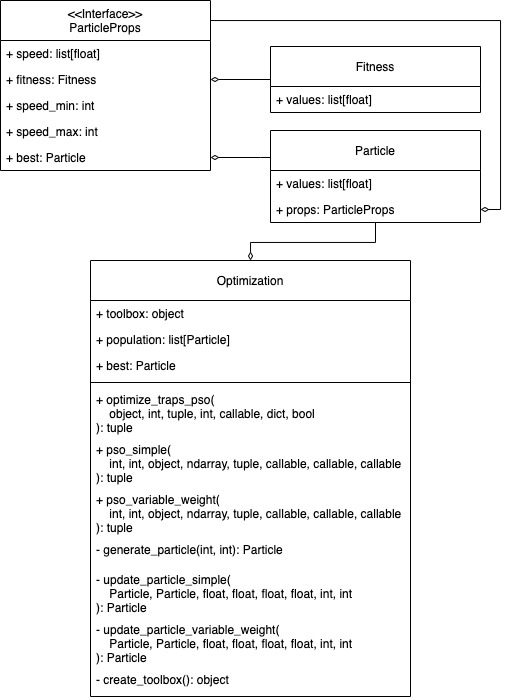
\includegraphics[width=\textwidth]{optimization-modules.jpeg}
    \caption{Diagrama de clases describiendo los módulos del sistema.}
    \label{fig:optimization-modules}
  \end{figure}

  \subsection{Integración con el paquete MGSurvE}

  Para terminar esta sección de descripción de la solución, a continuación se
  describe la integración del algoritmo propuesto al paquete MGSurvE. El
  paquete, al ya contar con una función de optimización entre sus
  herramientas, integrar un nuevo algoritmo con la misma funcionalidad no fue
  complicado ni laborioso. Se añadió una clase llamada $PSO$, la cual tiene
  una interfaz similar a la del algoritmo de GA actual de MGSurvE. Los
  argumentos que recibe el constructor de la clase son: landscape, el objeto
  del paquete MGSurvE que contiene información del entorno, trampas y
  migración de mosquitos; pop\_size, el tamaño de la población; generations,
  en donde se especifican el número de generaciones en las que el algoritmo
  correrá; speed\_min, la velocidad mínima de las partículas; speed\_max, la
  velocidad máxima de las partículas; phi1, límite superior para generar
  números aleatorios para influenciar la búsqueda local; phi2, límite superior
  para generar números aleatorios para influenciar la búsqueda global; w\_max,
  peso inercial máximo; y finalmente, w\_min, peso inercial mínimo.
  
  El PSO, además de ser compatible con la configuración del Landscape, también
  genera un logbook con los mismos datos generados por el GA, para así
  permitir la comparación de ambos métodos de optimización. 

\chapter{Metodología de evaluación}\label{chap:metolodogia}
\lhead{Capítulo 5. \emph{Metodología de evaluación}}

En este capítulo se describe la metodología de evaluación seleccionada para
validar que se ha resuelto la problemática identificada en este trabajo. A
continuación, se describe la técnica usada para evaluar el desempeño del
algoritmo implementado como solución, así como las métricas que se obtendrán
para confirmar la efectividad de la solución.

\section{Hardware}\label{sect:hardware}

  La evaluación del algoritmo propuesto en este trabajo se realizó en una
  MacBook Pro 2020, con un procesador Intel Core i7 de 2.6 GHz con 6 núcleos y
  memoria de 16 GB 2667 MHz DDR4.

\section{Selección de parámetros}

  Los algoritmos de tipo PSO necesitan una configuración de parámetros, como
  el tamaño de la población con la que se ejecutará la búsqueda y las
  velocidades mínima y máxima.

  Se realizó una búsqueda de parámetros comparando los resultados de ejecutar
  la optimización con un mismo entorno entorno y con distintas
  configuraciones de parámetros. La Tabla \ref{table:params-options} contiene
  las diferentes configuraciones con que el algoritmo de
  optimización fue ejecutado. Se ejecutó 5 veces un PSO con cada
  configuración, para así obtener promedios de los resultados arrojados
  por cada una. En la sección \ref{sect:busqueda-mejores-params} se explicarán
  a detalle los resultados de esta búsqueda.

  \begin{table}[ht!]
    \caption{Todas las opciones de parámetros}
    \begin{center}
      \begin{tabular}{|c|c|c|c|}
        \hline
        Configuración & Tamaño de población & Velocidad Mínima & Velocidad Máxima \\
        \hline
        1 & 12 & -5 & 5 \\
        \hline
        2 & 12 & -20 & 20 \\
        \hline
        3 & 40 & -5 & 5 \\
        \hline
        4 & 40 & -20 & 20 \\
        \hline
      \end{tabular}
      \label{table:params-options}
    \end{center}
  \end{table}

\section{Comparación de métodos}
  
  Se determinó que la mejor manera de evaluar el desempeño del algoritmo
  propuesto en este trabajo es una comparación directa entre el algoritmo PSO 
  y el algoritmo existente en MGSurvE. Para esto, primero se realizó una
  búsqueda de mejores parámetros, para así tener una referencia de con qué
  tipo de parámetros el algoritmo PSO funciona mejor. Después, con los mejores
  parámetros encontrados, se comparará contra el GA en un entorno generado por
  el mismo MGSurvE. A continuación se detallará todo el procedimiento. 

  \subsection{Generación del entorno de evaluación}

  Para generar el entorno de evaluación se utilizó la función $ptsDonut$ de
  MGSurvE, la cual genera una distribución de puntos en forma de dona. Como
  parámetros, se le indicó que generara 200 puntos en un radio mínimo de la
  dona de 75 unidades y un máximo de 100 unidades. El resultado de ejecutar
  esta función es el mostrado en la Figura \ref{fig:evaluation-env}. Este
  entorno cuenta con 4 trampas, cuyas ubicaciones serán optimizadas. Para
  facilitar el uso de este entorno, se guardaron los datos generados por
  MGSurvE en un archivo pickle, para después ser cargado por el programa de
  comparación de métodos. 

  \begin{figure}[ht!]
    \centering
    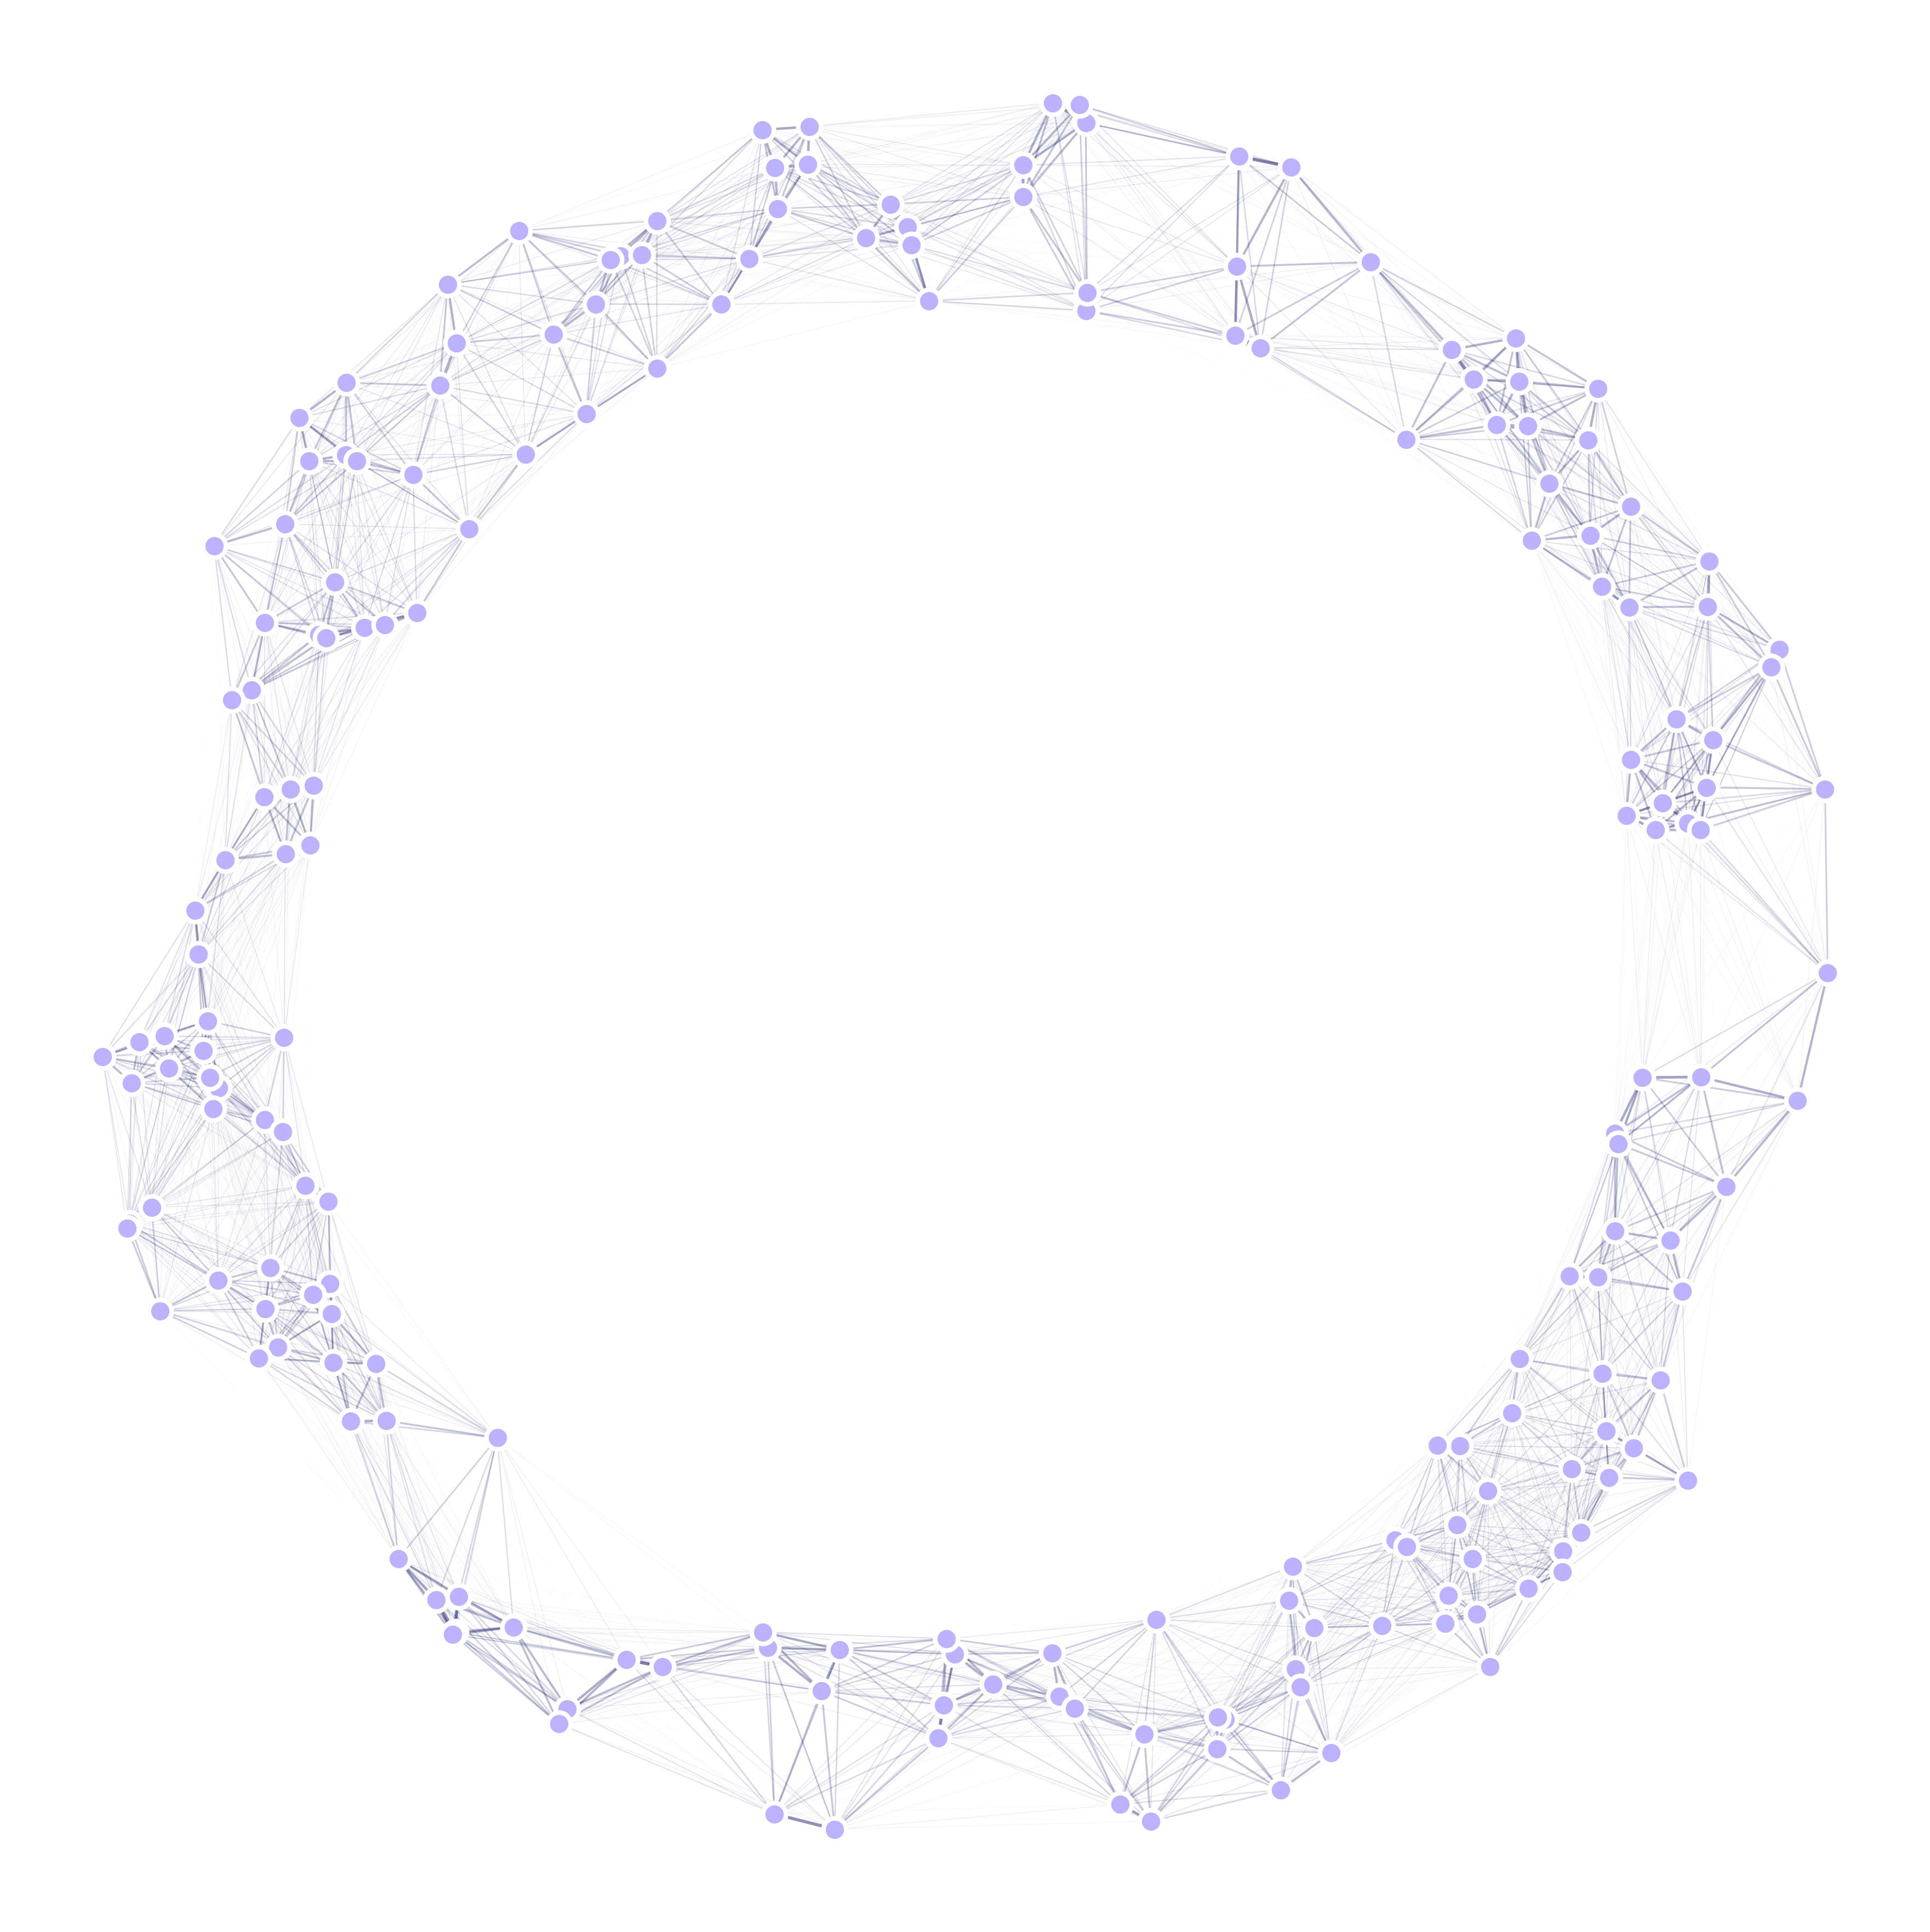
\includegraphics[width=\textwidth]{eval-env.png}
    \caption{Entorno generado para la evaluación del algoritmo PSO.}
    \label{fig:evaluation-env}
  \end{figure}

  \subsection{Ejecución de optimizaciones}

  Para facilitar la ejecución de ambos algoritmos con un mismo entorno, se
  escribió un programa que primero lee la información del entorno generado
  previamente, para después correr los dos métodos de optimización (PSO y
  GA). Este programa ejecuta 20 veces el PSO y 20 veces el GA, para así
  obtener mejores estadísticas de los datos generados (como los promedios, y
  percentiles). Los datos generados por el programa se almacenaron en
  estructuras de datos para, posteriormente, generar visualizaciones de estos.

  \subsection{Métricas}

  Una vez exportados los datos de las optimizaciones, se obtuvieron tres
  métricas que ayudan a validar el desempeño del algoritmo propuesto en este
  trabajo: tiempo de ejecución de la optimización, esto ayuda a verificar si
  el algoritmo PSO es más rápido que la implementación actual en MGSurvE;
  generación en la que se encuentra el valor óptimo, así se sabe qué algoritmo
  encuentra el valor mínimo más rápido; y valor mínimo de detección de
  mosquitos, esta métrica es la principal para saber si el PSO es mejor
  optimizando las ubicaciones de las trampas a comparación del GA y
  determinará si se cumplió el objetivo.

  En el siguiente capítulo se presentan los resultados obtenidos de esta
  evaluación.

\chapter{Resultados}\label{chap:resultados}
\lhead{Capítulo 6. \emph{Resultados}}
En este capítulo se describirán a detalle los resultados obtenidos de la
evaluación del algoritmo PSO presentado en este trabajo.

\section{Búsqueda de mejores parámetros}\label{sect:busqueda-mejores-params}
  Los resultados de la búsqueda de mejor configuración para el PSO se muestran
  en la tabla \ref{table:params-results}. En negrita se resalta la
  configuración con el mejor promedio de resultados. Como se puede ver en la
  tabla, la configuración 4 de parámetros fue la que arrojó un mejor valor
  mínimo de detección de mosquitos, seguida de cerca por la configuración 2,
  enseguida la 3 y muy por detrás la configuración 1. La principal causa de
  que la configuración 1 y 2 obtuvieran resultados muy similares son las
  velocidades mínima y máxima, pues ocasionan búsquedas amplias al inicio del
  algoritmo, encontrando así los mínimos globales rápidamente. Sin embargo,
  hay una gran diferencia de más de 45 segundos en el tiempo de ejecución
  promedio, esto debido a la diferencia entre el tamaño de población.

  Para comprender y analizar mejor el comportamiento de cada configuración,
  se presenta la Figura \ref{fig:params-search-lines}, en la cual se grafica
  el comportamiento del PSO con cada configuración. En esta gráfica se
  aprecian 5 líneas por cada configuración, para así entender su
  comportamiento general. En la gráfica que se ve la similitud entre las
  configuraciones 2 y 4, sin embargo, la configuración 4 comienza a encontrar
  mejores resultados que la 2 en menos generaciones. Así mismo, se aprecia en
  la gráfica que las configuraciones 2 y 4 se atoran en menos mínimos locales,
  y la configuración 4 lo hace menos que la 2.

  Por lo tanto, se seleccionaron 20 y -20 como velocidad máxima y mínima.
  Igualmente, como población para la etapa de comparación contra el algoritmo
  genético se optó por 40 partículas, pues se obtuvieron mejores resultados en
  menor cantidad de generaciones con este tamaño de población. Además, como
  parámetros de peso ($w$) máximo y mínimo se seleccionaron 1.5 y 0.9, para
  lograr aún mejores búsquedas globales al principio del algoritmo y mejores
  búsquedas locales en las etapas finales. Para las generaciones, se puede
  apreciar en la Figura \ref{fig:params-search-lines} que entre más
  generaciones, mejores son los resultados, por esto, se usarán 500
  generaciones para la comparación de algoritmos.
  
  \begin{table}[ht!]
    \caption{
      Resultados de comparación de las diferentes configuraciones de
      parámetros para el PSO (Tabla \ref{table:params-options}).
    }
    \begin{center}
      \begin{tabular}{|c|c|c|}
        \hline
        Configuración & Resultado promedio (días) & Tiempo de ejecución
          promedio (segundos) \\
        \hline
        1 & 1.654883190977614 & 15.095740842819215 \\
        \hline
        2 & 1.5887967821719775 & 15.379290246963501 \\
        \hline
        3 & 1.5999659131506383 & 50.010193014144896 \\
        \hline
        4 & \bfseries 1.5770302194541654 & 60.24051342010498 \\
        \hline
      \end{tabular}
      \label{table:params-results}
    \end{center}
  \end{table}

  \begin{figure}[ht!]
    \centering
    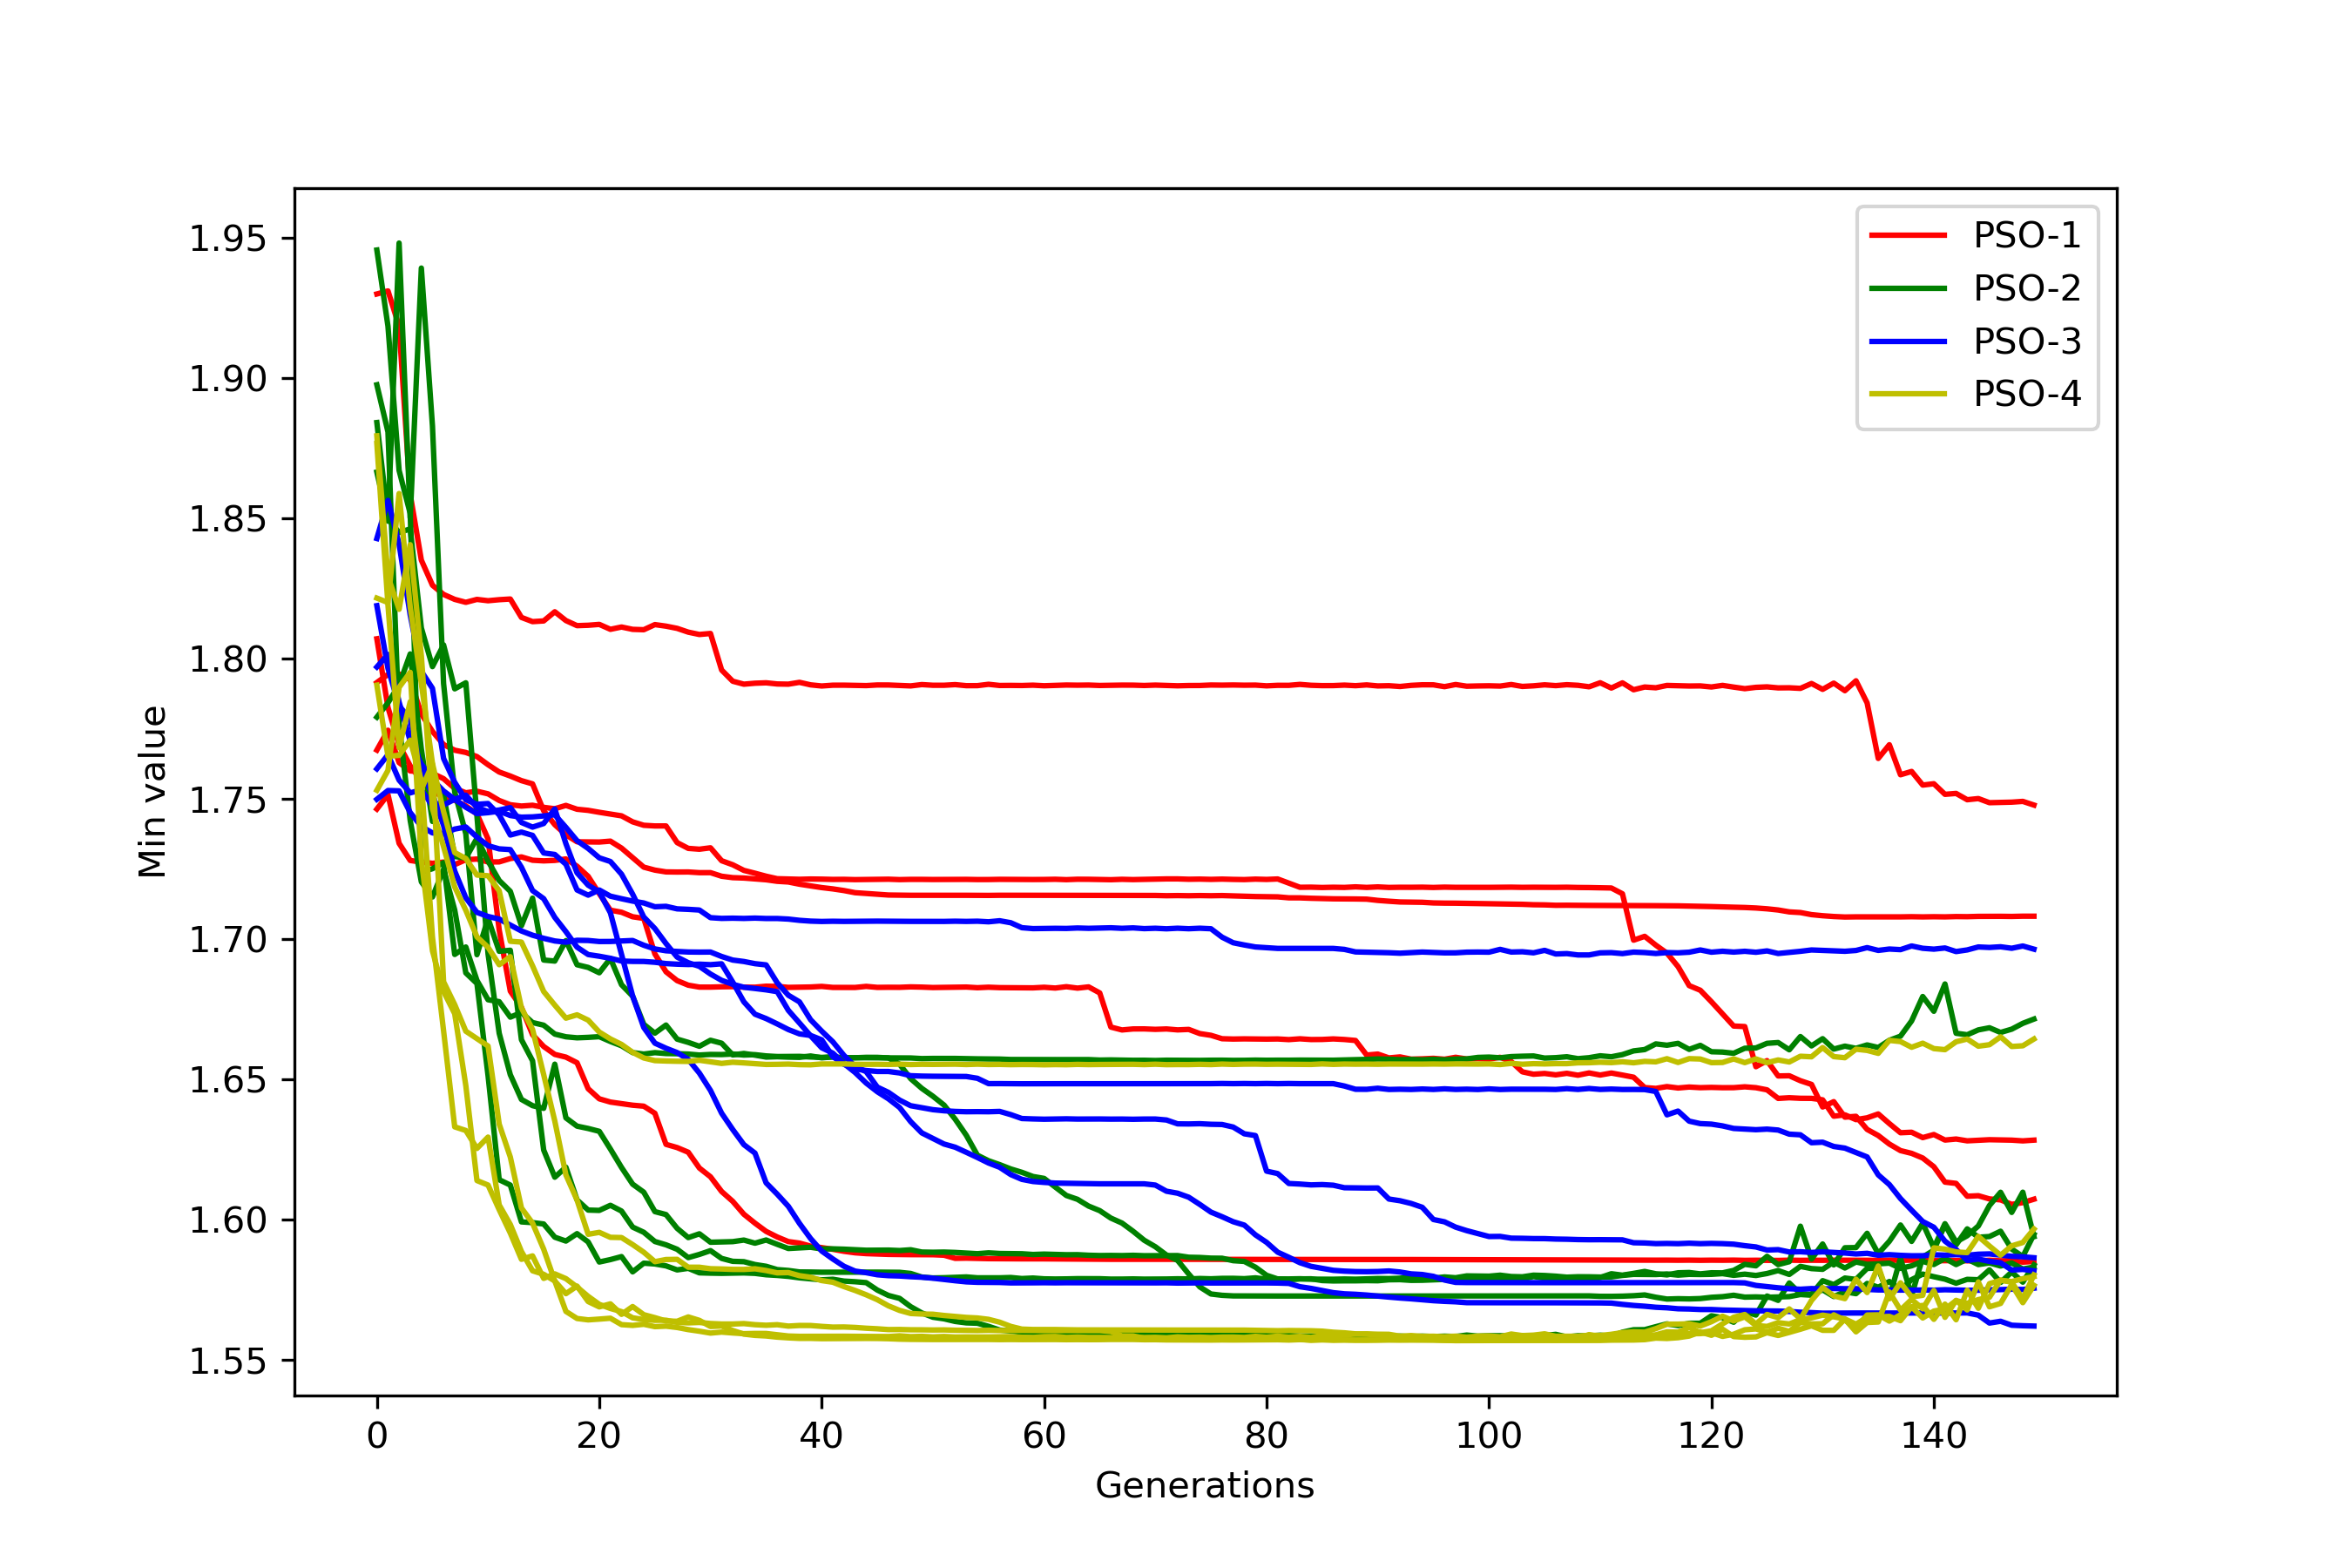
\includegraphics[width=\textwidth]{params-search-lines.png}
    \caption{
      Comportamiento del PSO con diferentes configuraciones. En rojo se
      muestran las ejecuciones de la configuración 1; en verde la
      configuración 2; en azul la configuración 3; y en amarillo la 4.
    }
    \label{fig:params-search-lines}
  \end{figure}

\section{Comparación de algoritmos}

  En las Figuras \ref{fig:average-results} y \ref{fig:percentile} se presentan
  los comportamientos generales de cada algoritmo con el entorno generado
  previamente. En la primer imagen se muestran los resultados óptimos
  encontrados por generación durante las 20 ejecuciones de cada algoritmo. Se
  puede apreciar como, el PSO, es capaz de encontrar muy buenos resultados
  tempranamente, pues entre las generaciones 50 y 100 está alcanzando los
  mínimos. Sin embargo, un 20\% de las ocasiones, el algoritmo propuesto se
  encuentra atorado en mínimos locales desde etapas tempranas de la búsqueda y
  no es capaz de salir. A diferencia del PSO, el algoritmo genético es capaz
  de salir de los mínimos locales y encontrar un valor cercano al mínimo
  global en las etapas tardías de la optimización. A pesar de esto, el PSO
  logra encontrar mejores resultados la mayoría de las veces.

  \begin{figure}[ht!]
    \centering
    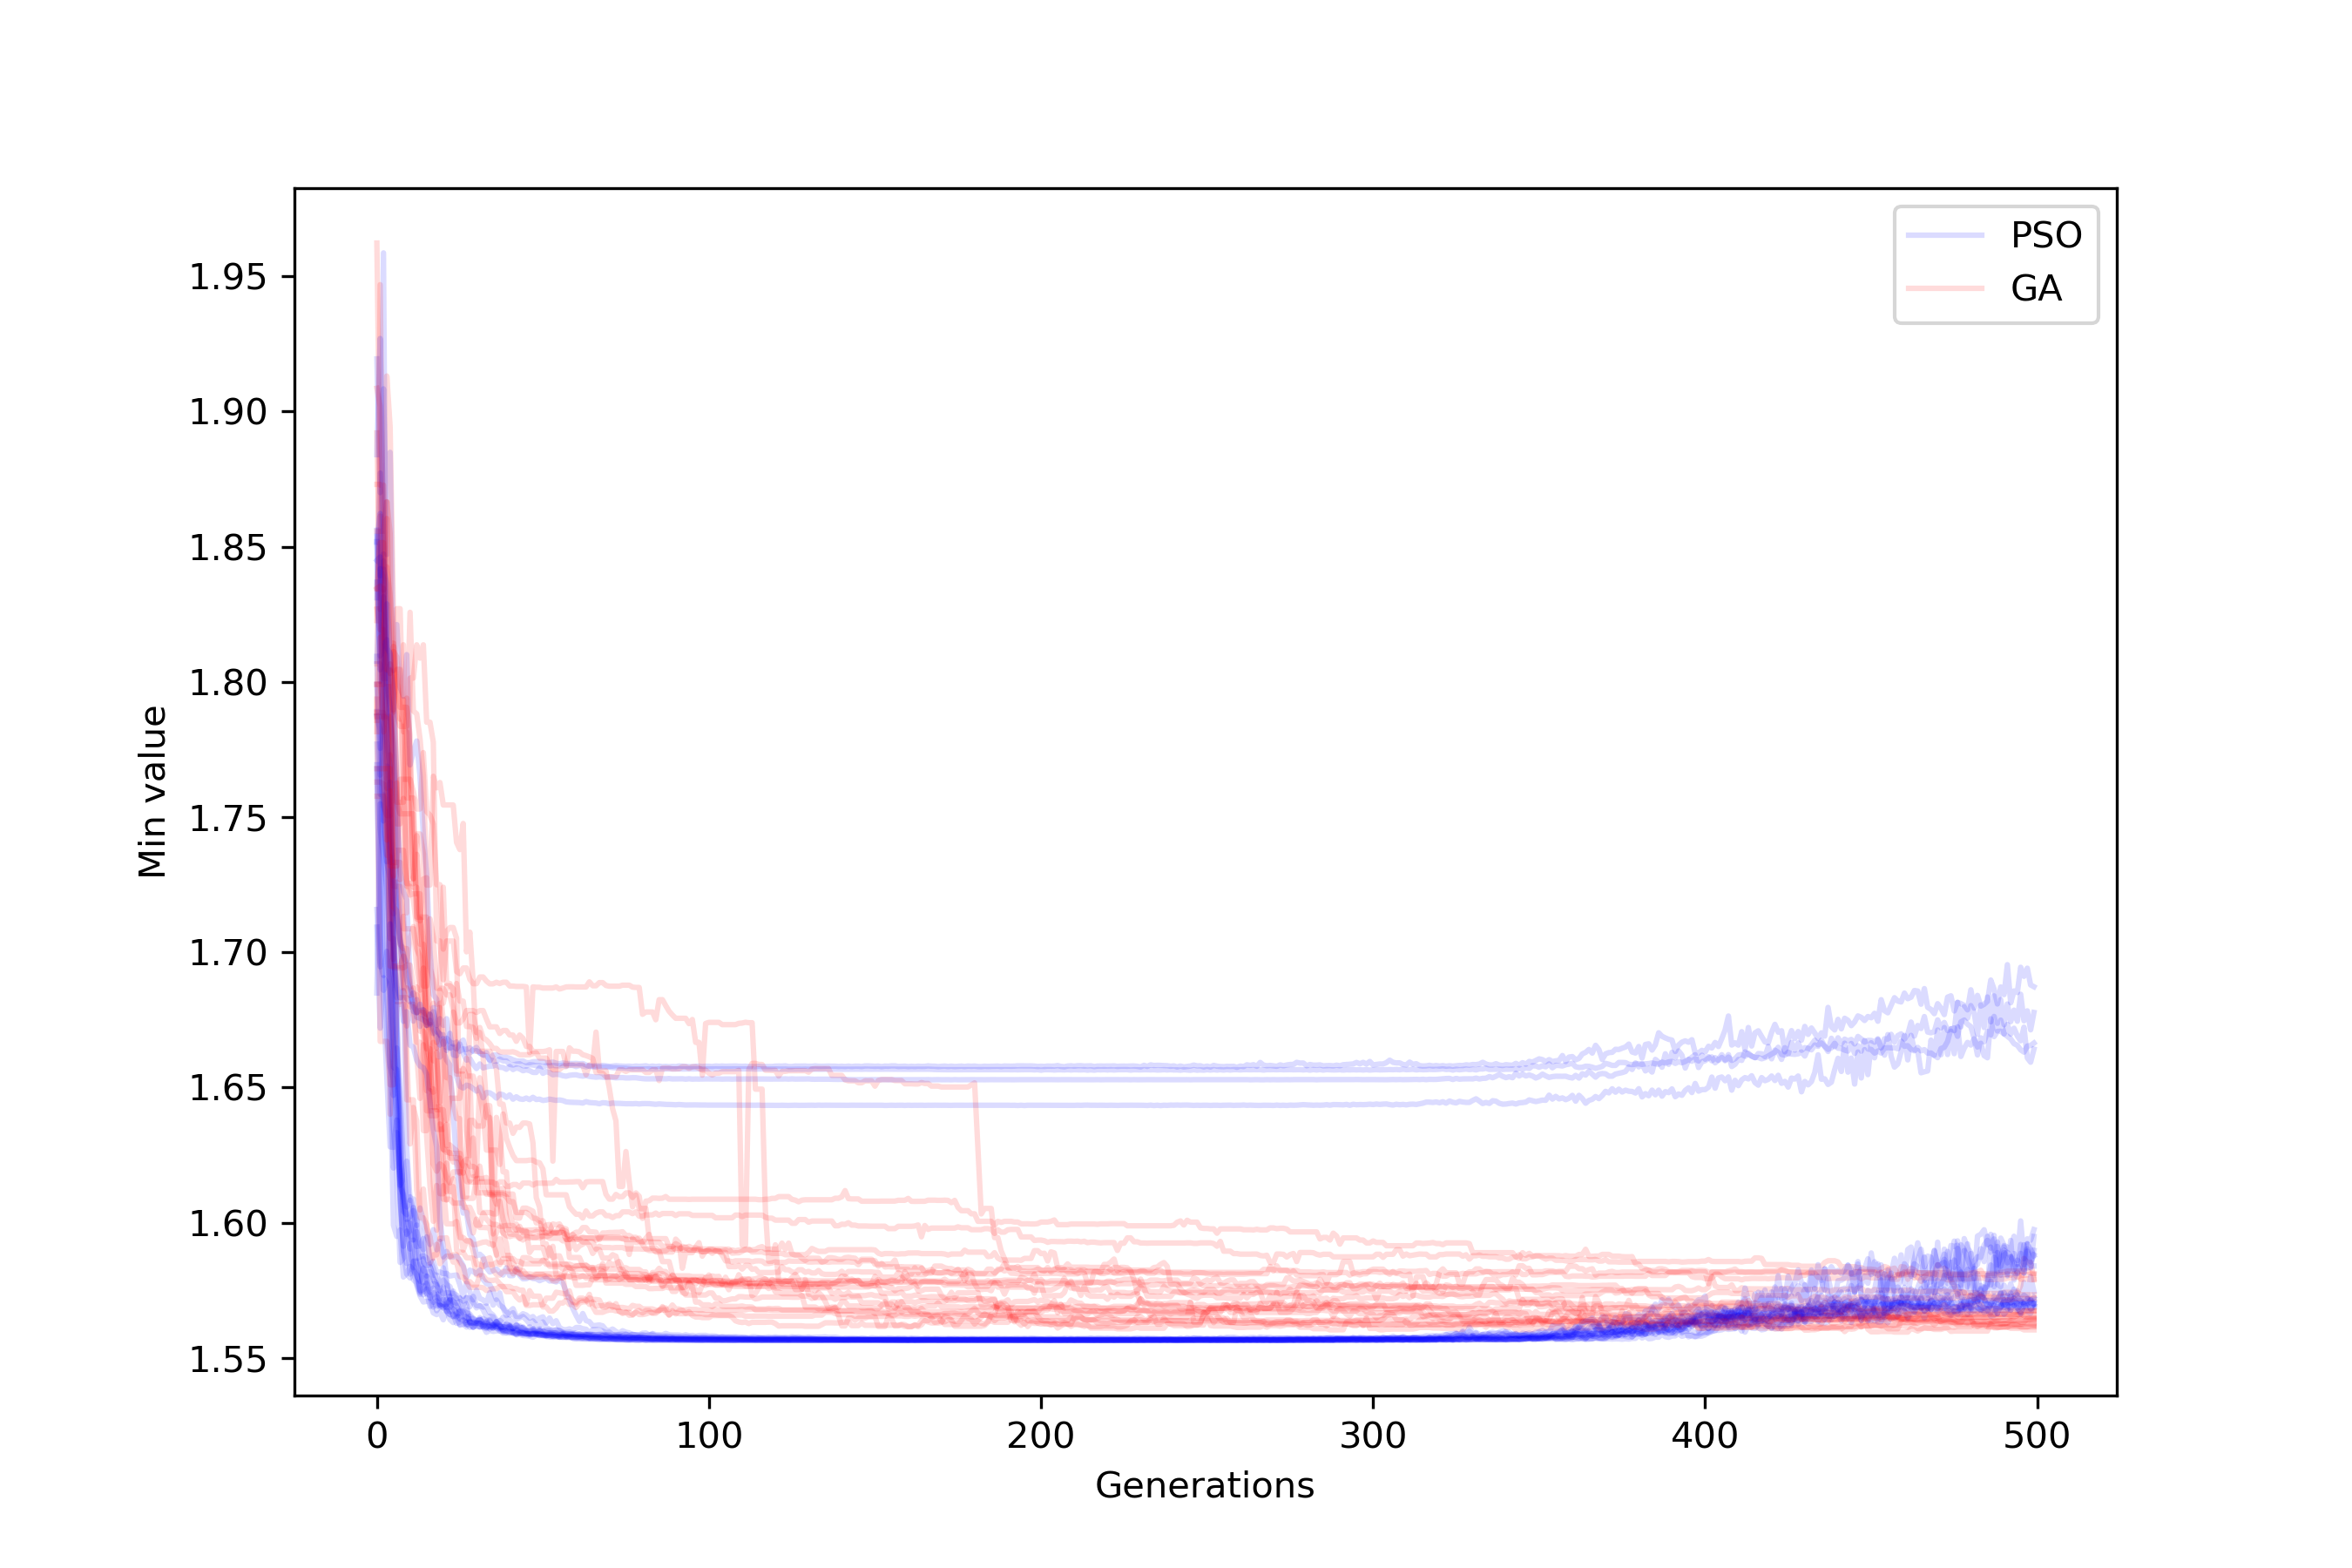
\includegraphics[width=\textwidth]{average-results.png}
    \caption{Comportamiento de PSO y GA}
    \label{fig:average-results}
  \end{figure}

  En la figura \ref{fig:percentile} se puede apreciar mejor la calidad de los
  resultados encontrados por cada algoritmo. En la gráfica de bandas de
  percentiles se muestra una línea sólida con el promedio de los resultados
  por generación y en colores más claros se presentan los percentiles 75 y 25.
  Se puede apreciar que la mayoría de las veces el PSO logra optimizar de
  mejor manera la posición de las trampas en el entorno generado. La línea de
  promedio del PSO se ve separada de los percentiles debido a las ejecuciones
  en donde este algoritmo se vió atorado en un mínimo local.

  El tiempo de ejecución promedio del GA fue de 97.807 segundos con el equipo
  de cómputo presentado anteriormente (\ref{sect:hardware}) y el PSO presenta
  un tiempo de ejecución de 200.9426 segundos. El tiempo de ejecución del PSO
  se ve impactado en su mayoría por el número de evaluaciones por generación
  (40), a diferencia del GA (de 30 a 50). Además, la implementación del PSO
  realiza operaciones a nivel de Python, cuando el GA realiza la mayoría de
  sus operaciones de una manera más eficiente (con NumPy principalmente).

  Adicionalmente, en las Figuras \ref{fig:pso-best} y \ref{fig:ga-best} se
  presentan las mejores posiciones encontradas para las trampas por el PSO y
  el GA (respectivamente). Así mismo, las Figuras \ref{fig:pso-worst} y
  \ref{fig:ga-worst} muestran los peores resultados de estos algoritmos. En la
  Figura \ref{fig:pso-worst} se puede apreciar la consecuencia de quedar en un
  mínimo local, pues el resultado es significativamente peor que el del GA. 

  Gracias a estos resultados, se puede afirmar que el algoritmo propuesto en
  este trabajo logra encontrar mejores posiciones para las trampas, a
  comparación del algoritmo genético implementado en MGSurvE.

  \begin{figure}[ht!]
    \centering
    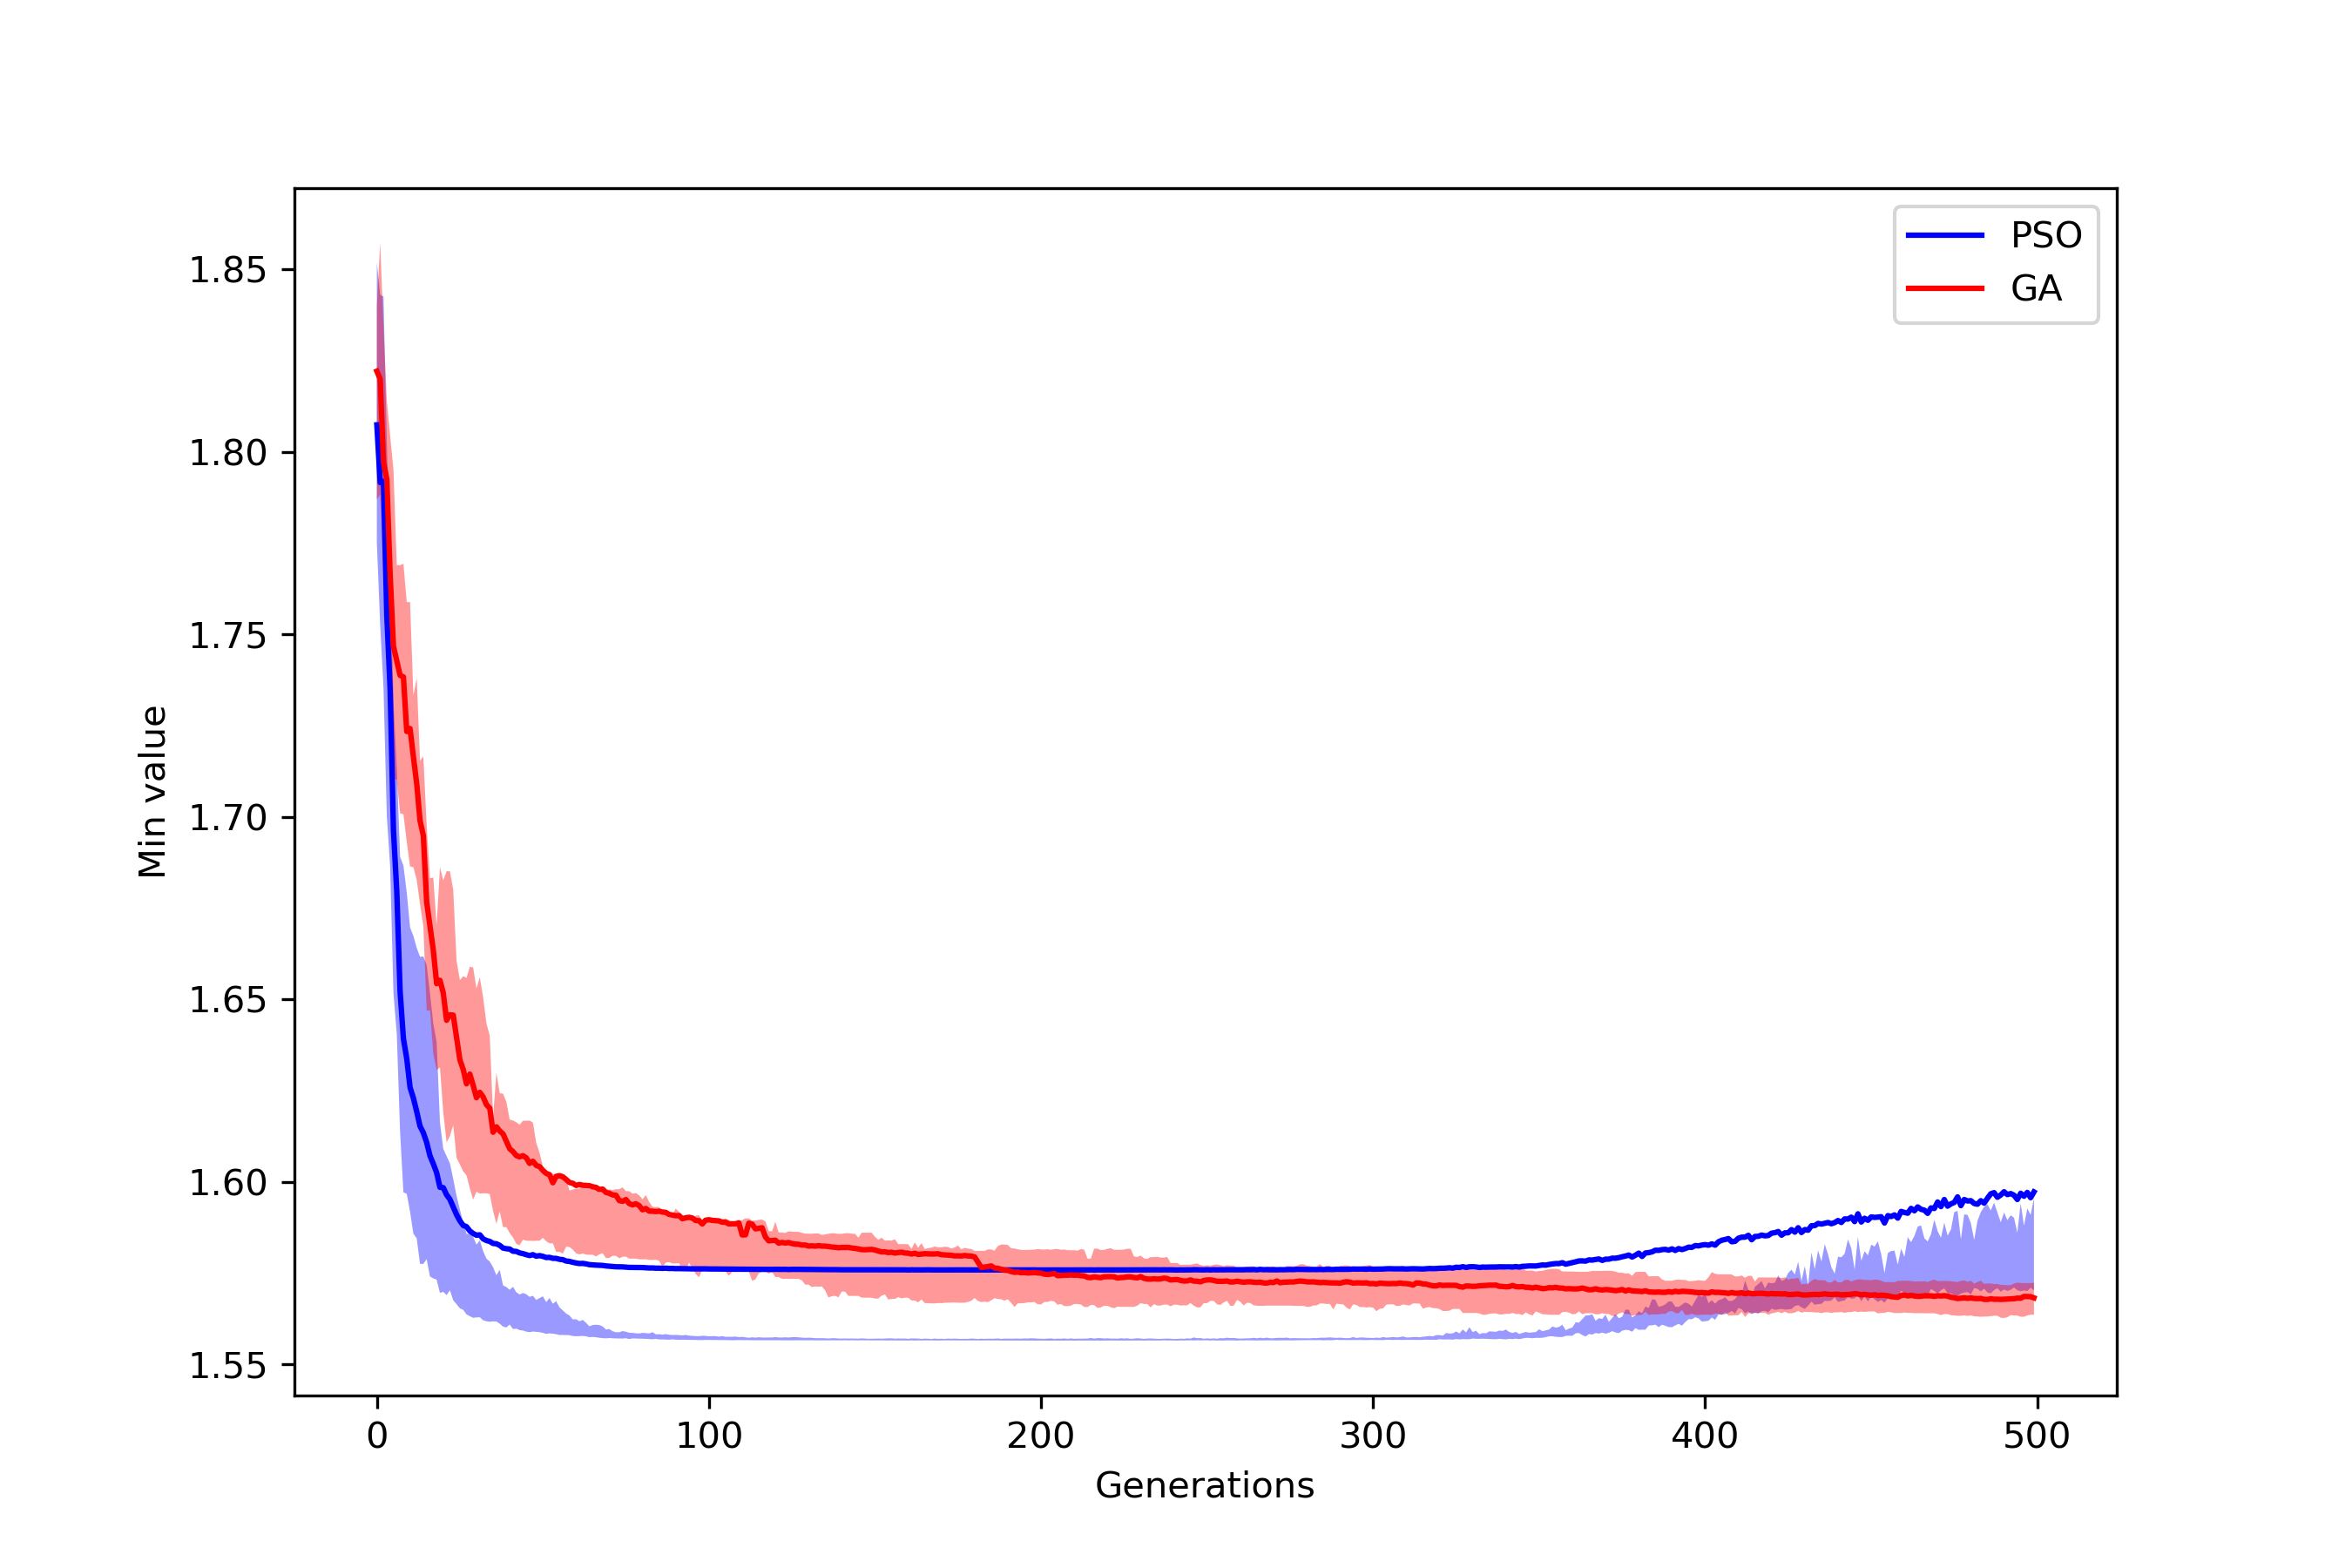
\includegraphics[width=\textwidth]{percentile.png}
    \caption{Bandas de percentiles de resultados de PSO y GA}
    \label{fig:percentile}
  \end{figure}

  \begin{figure}[ht!]
    \centering
    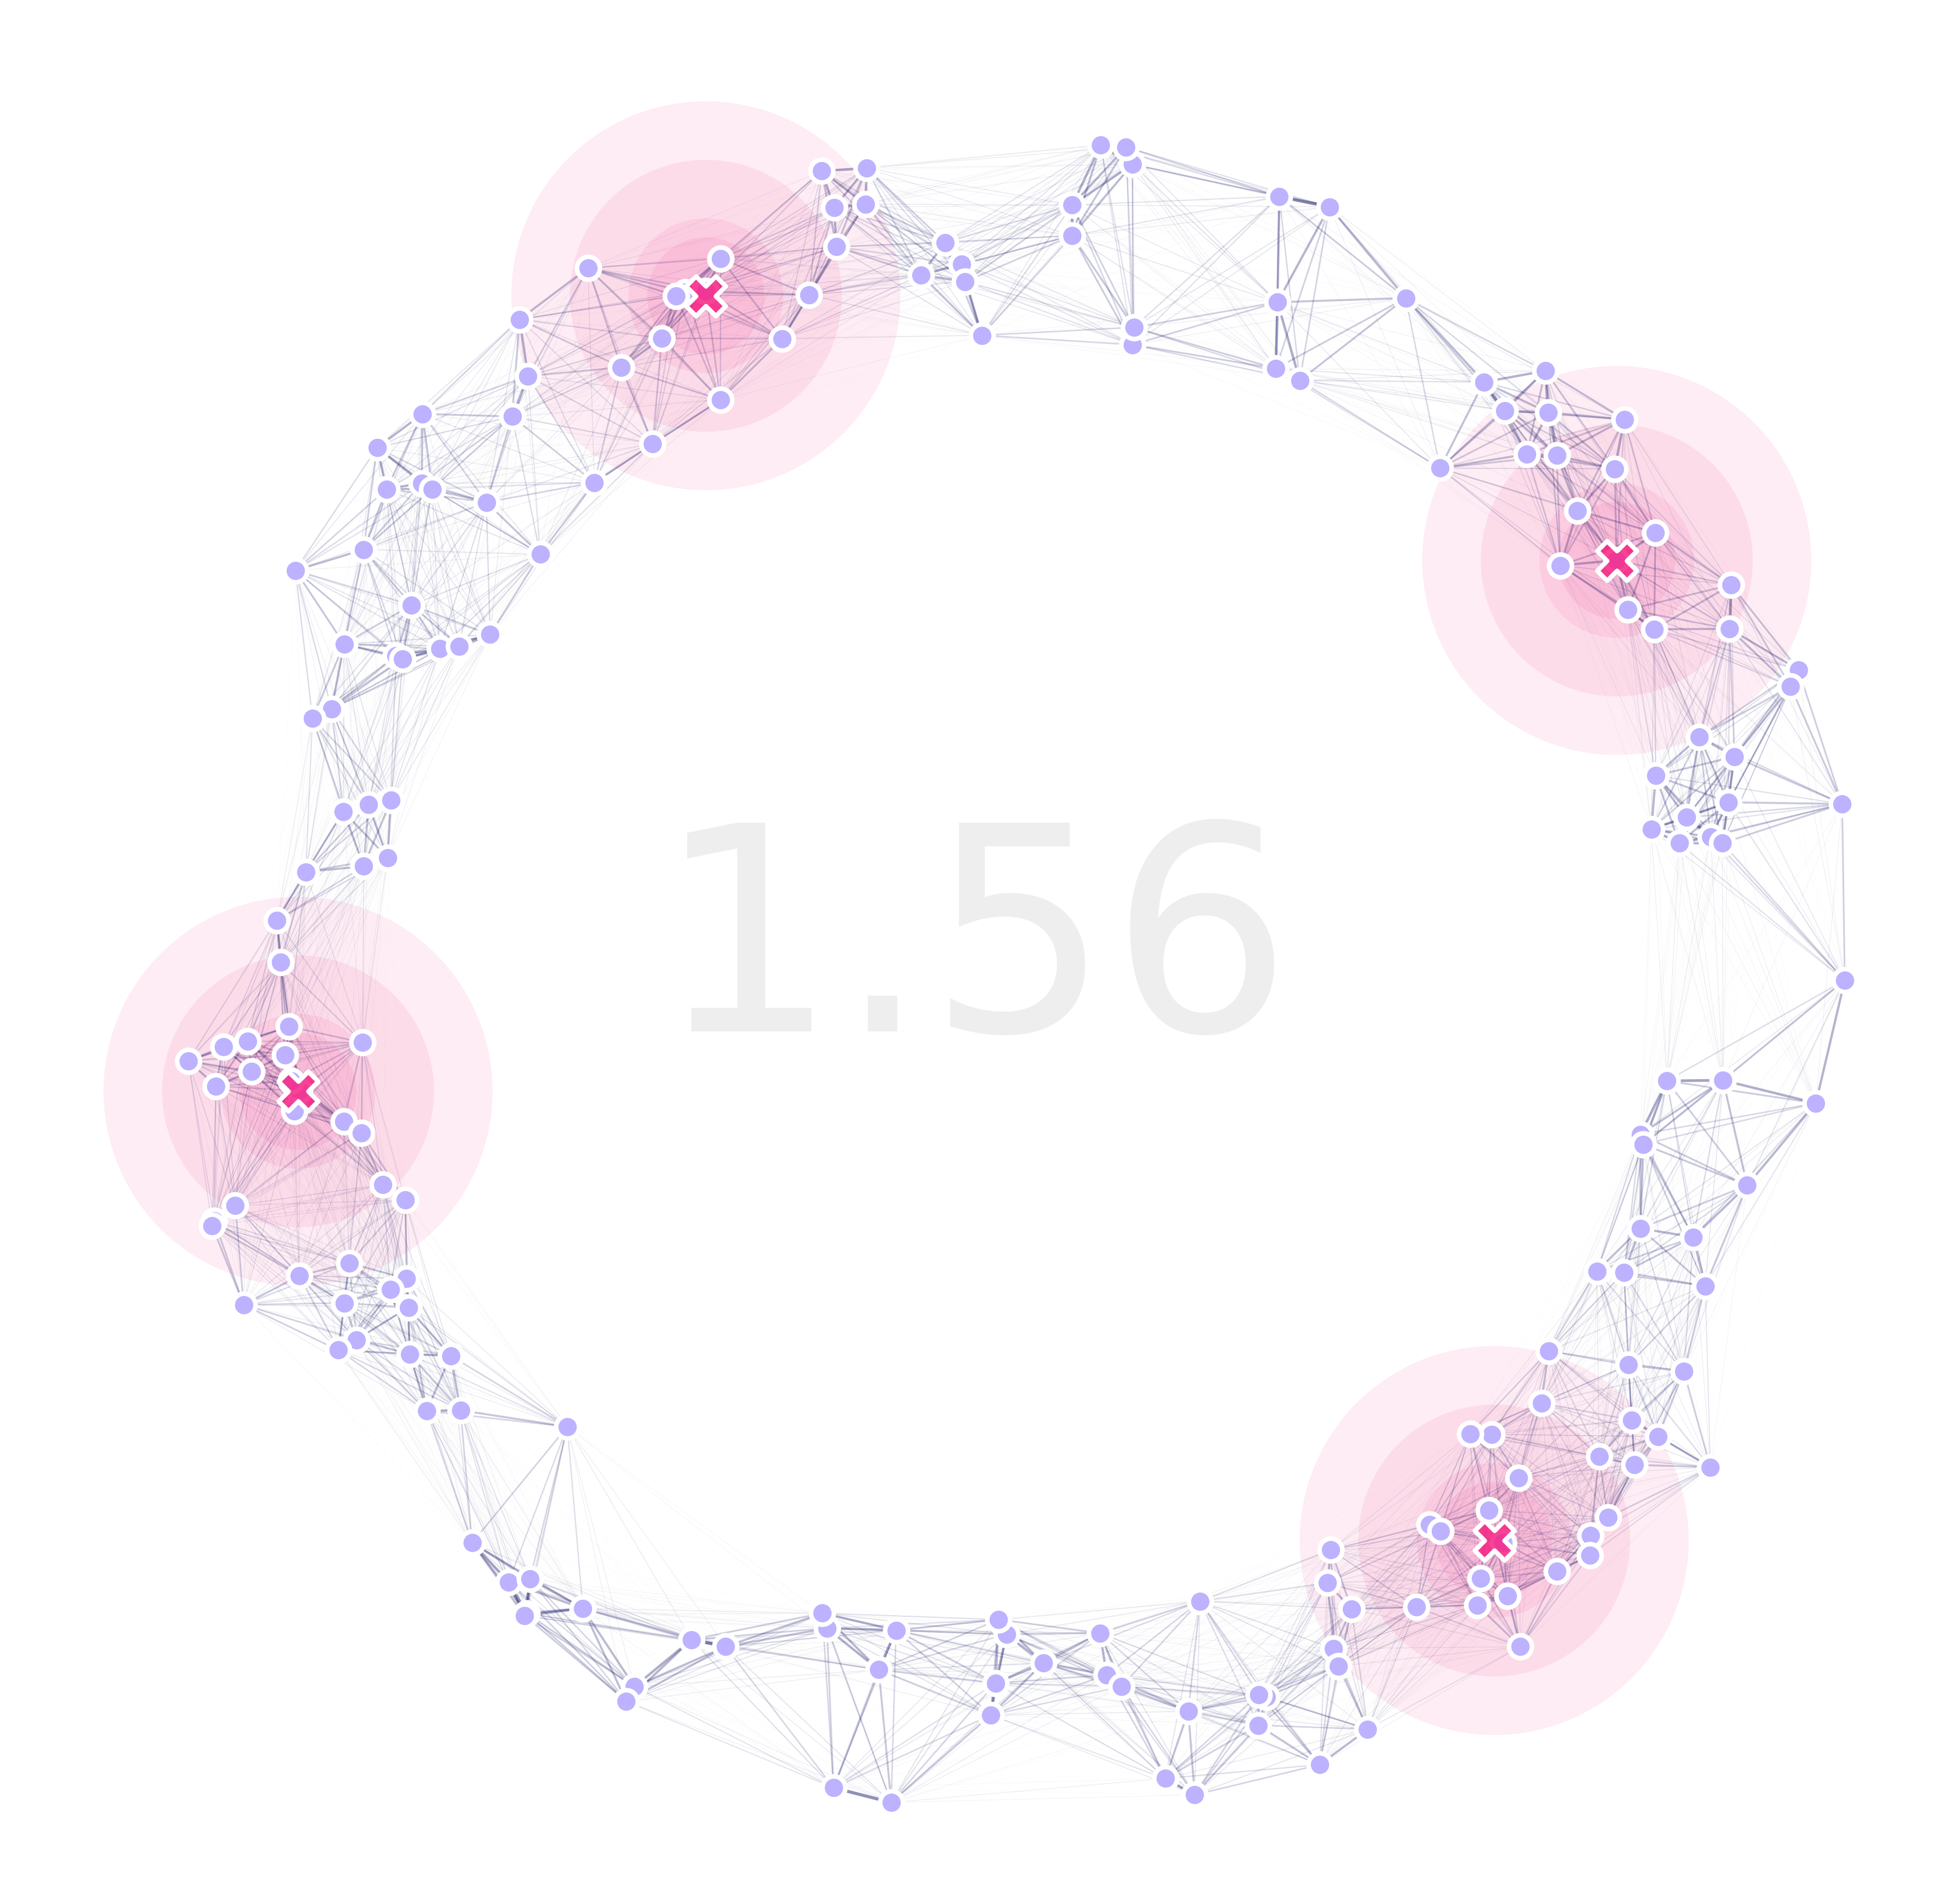
\includegraphics[width=\textwidth]{pso-best.png}
    \caption{Mejor resultado PSO}
    \label{fig:pso-best}
  \end{figure}

  \begin{figure}[ht!]
    \centering
    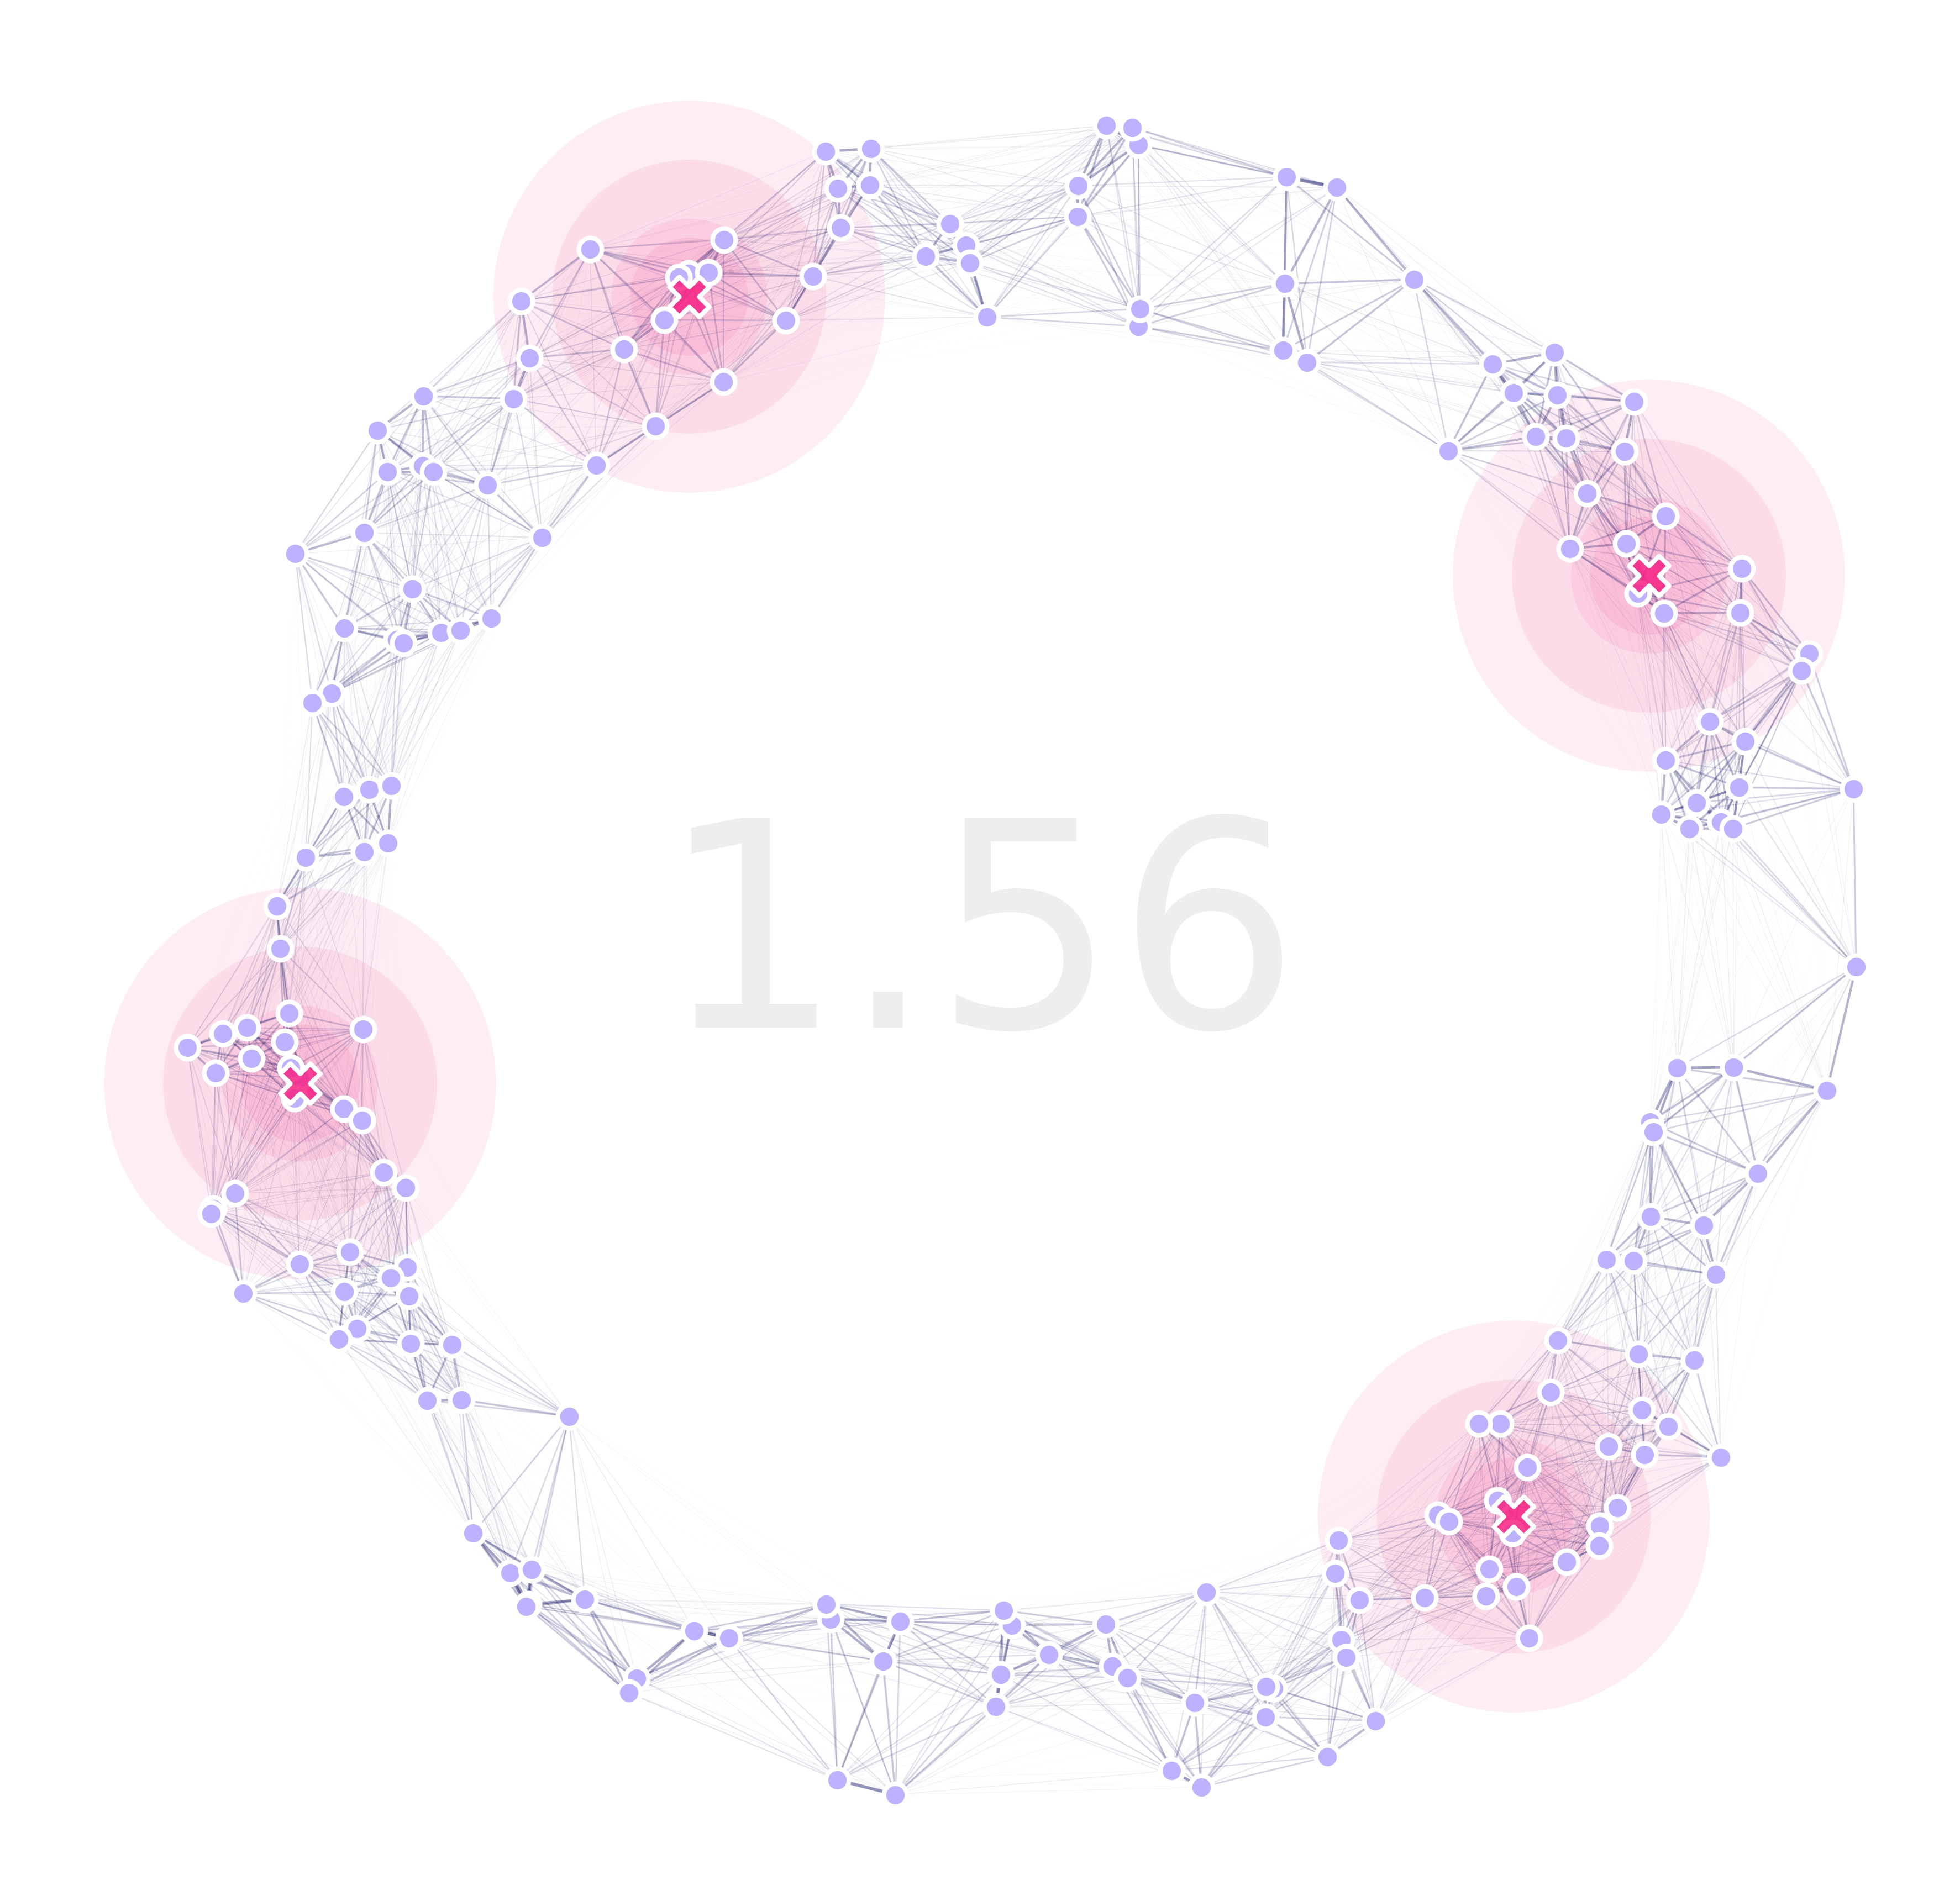
\includegraphics[width=\textwidth]{ga-best.png}
    \caption{Mejor resultado GA}
    \label{fig:ga-best}
  \end{figure}

  \begin{figure}[ht!]
    \centering
    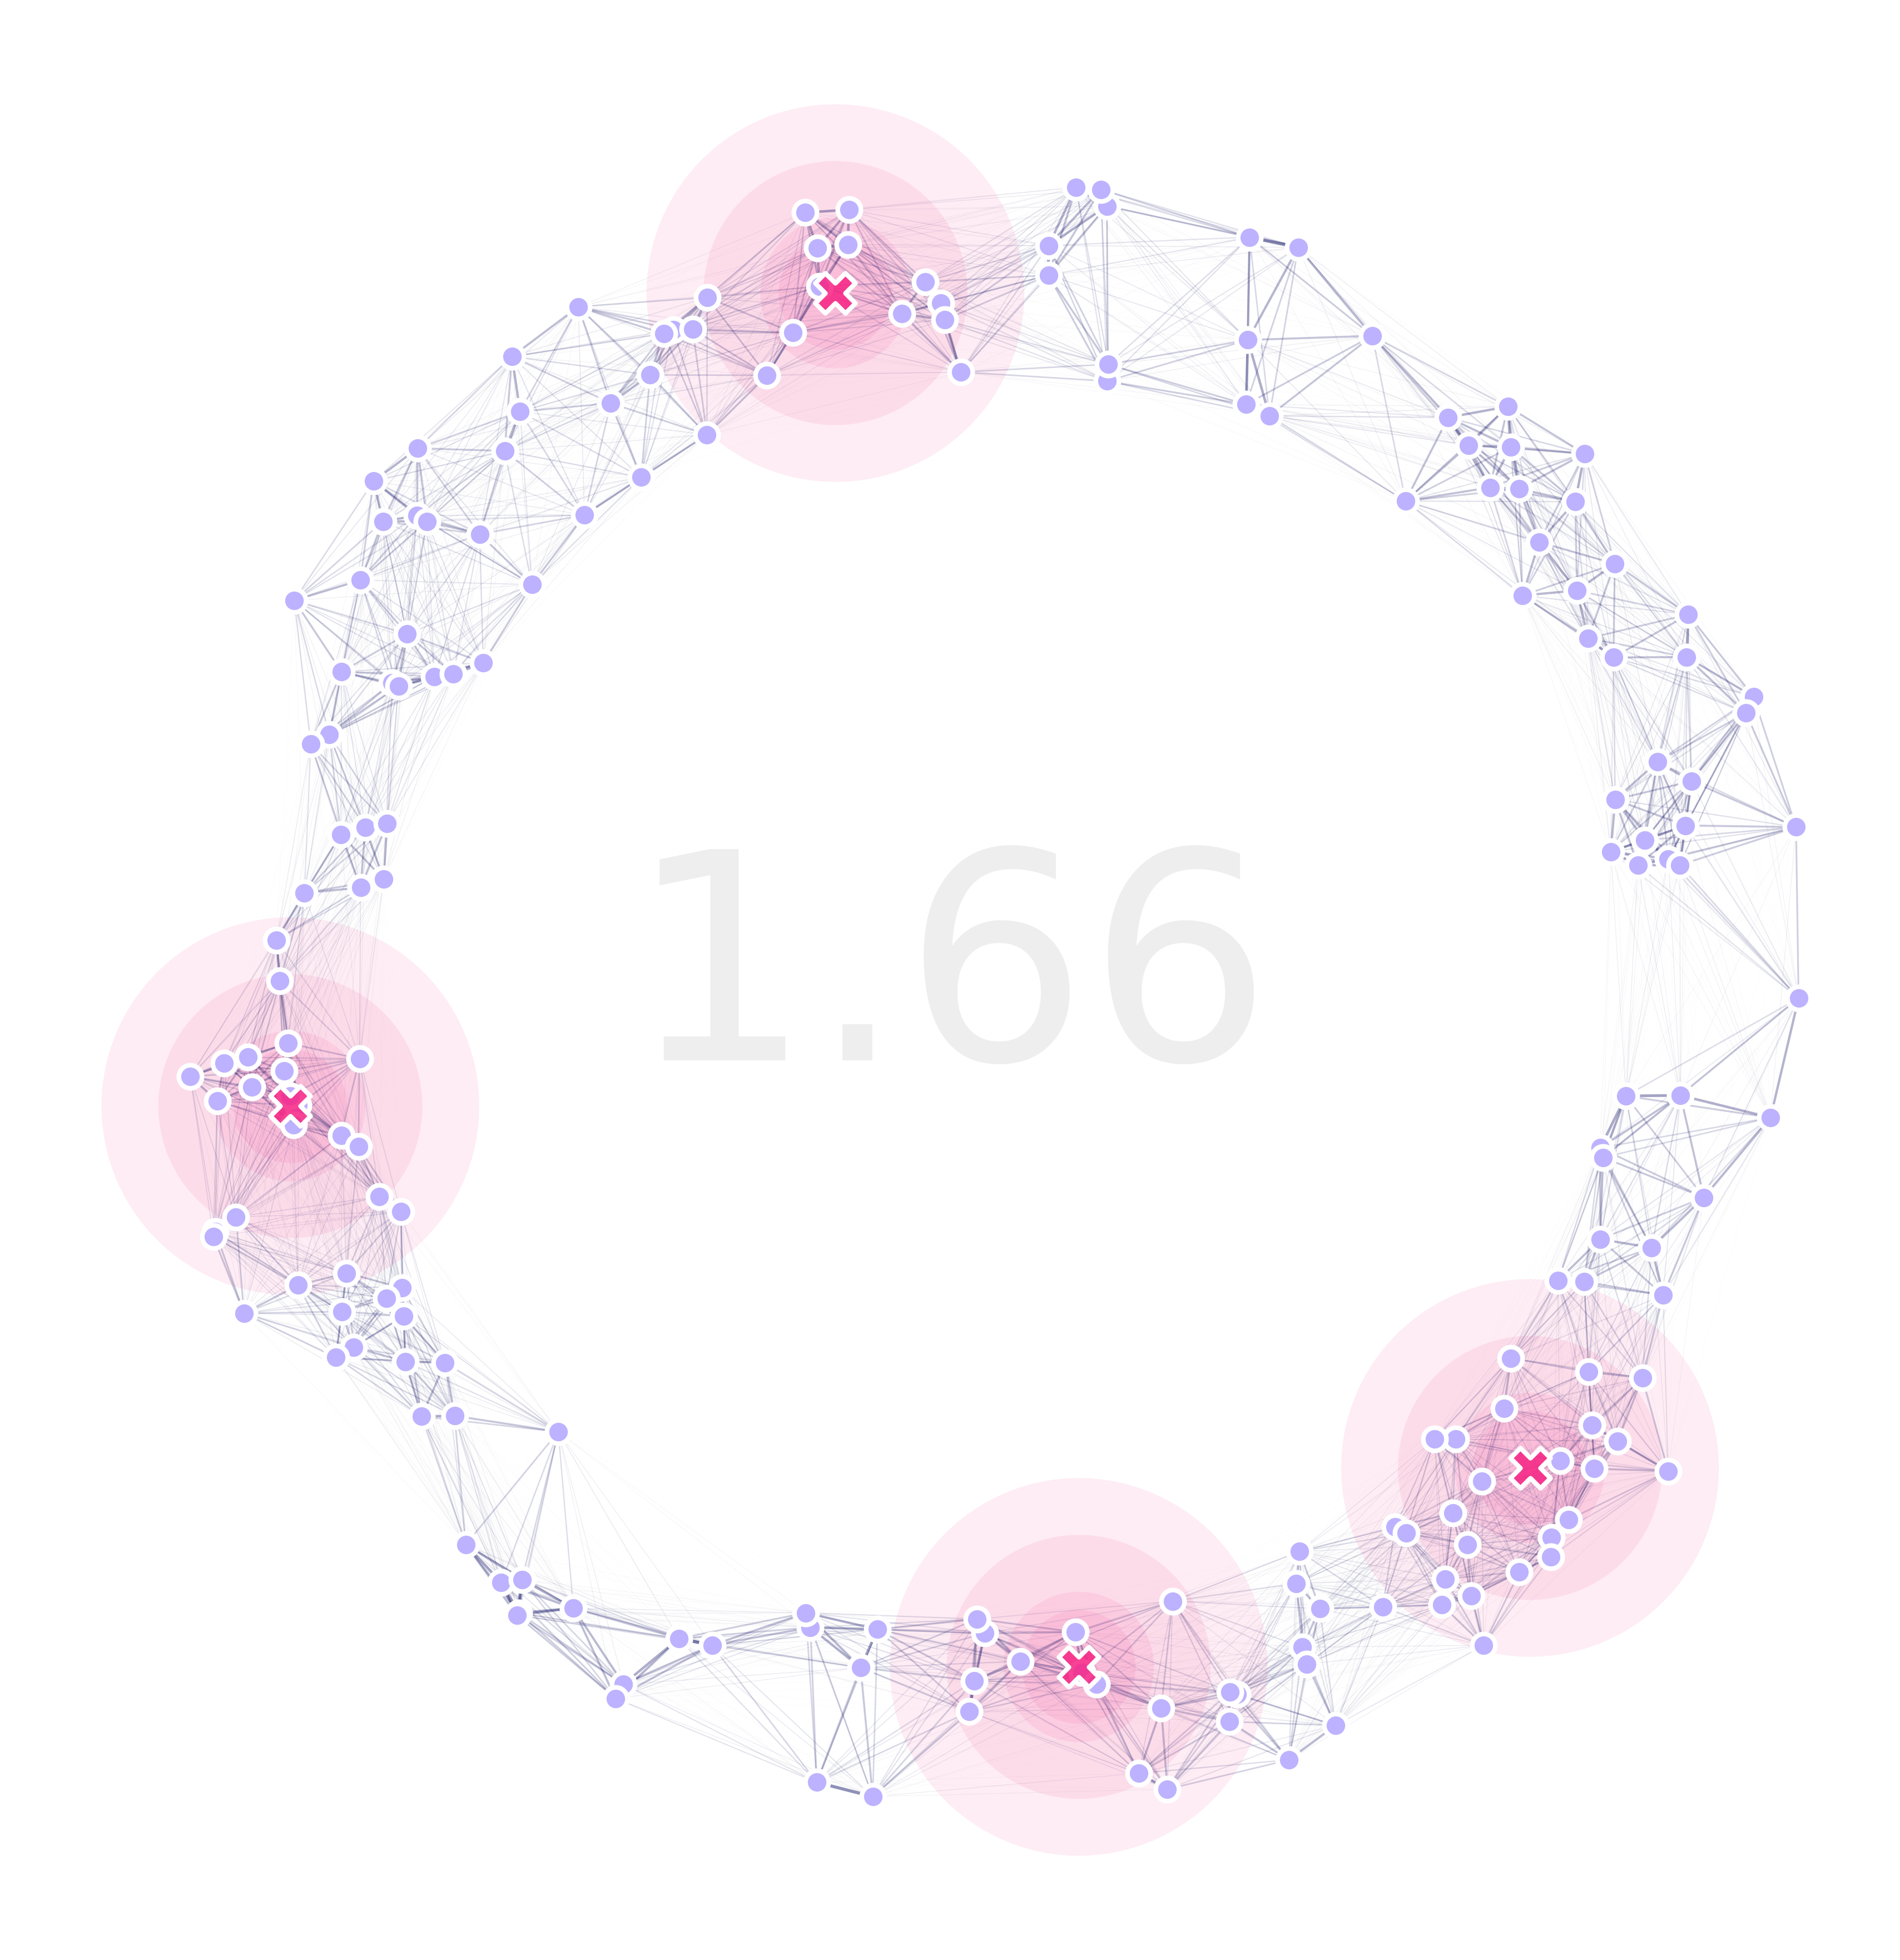
\includegraphics[width=\textwidth]{pso-worst.png}
    \caption{Peor resultado PSO}
    \label{fig:pso-worst}
  \end{figure}

  \begin{figure}[ht!]
    \centering
    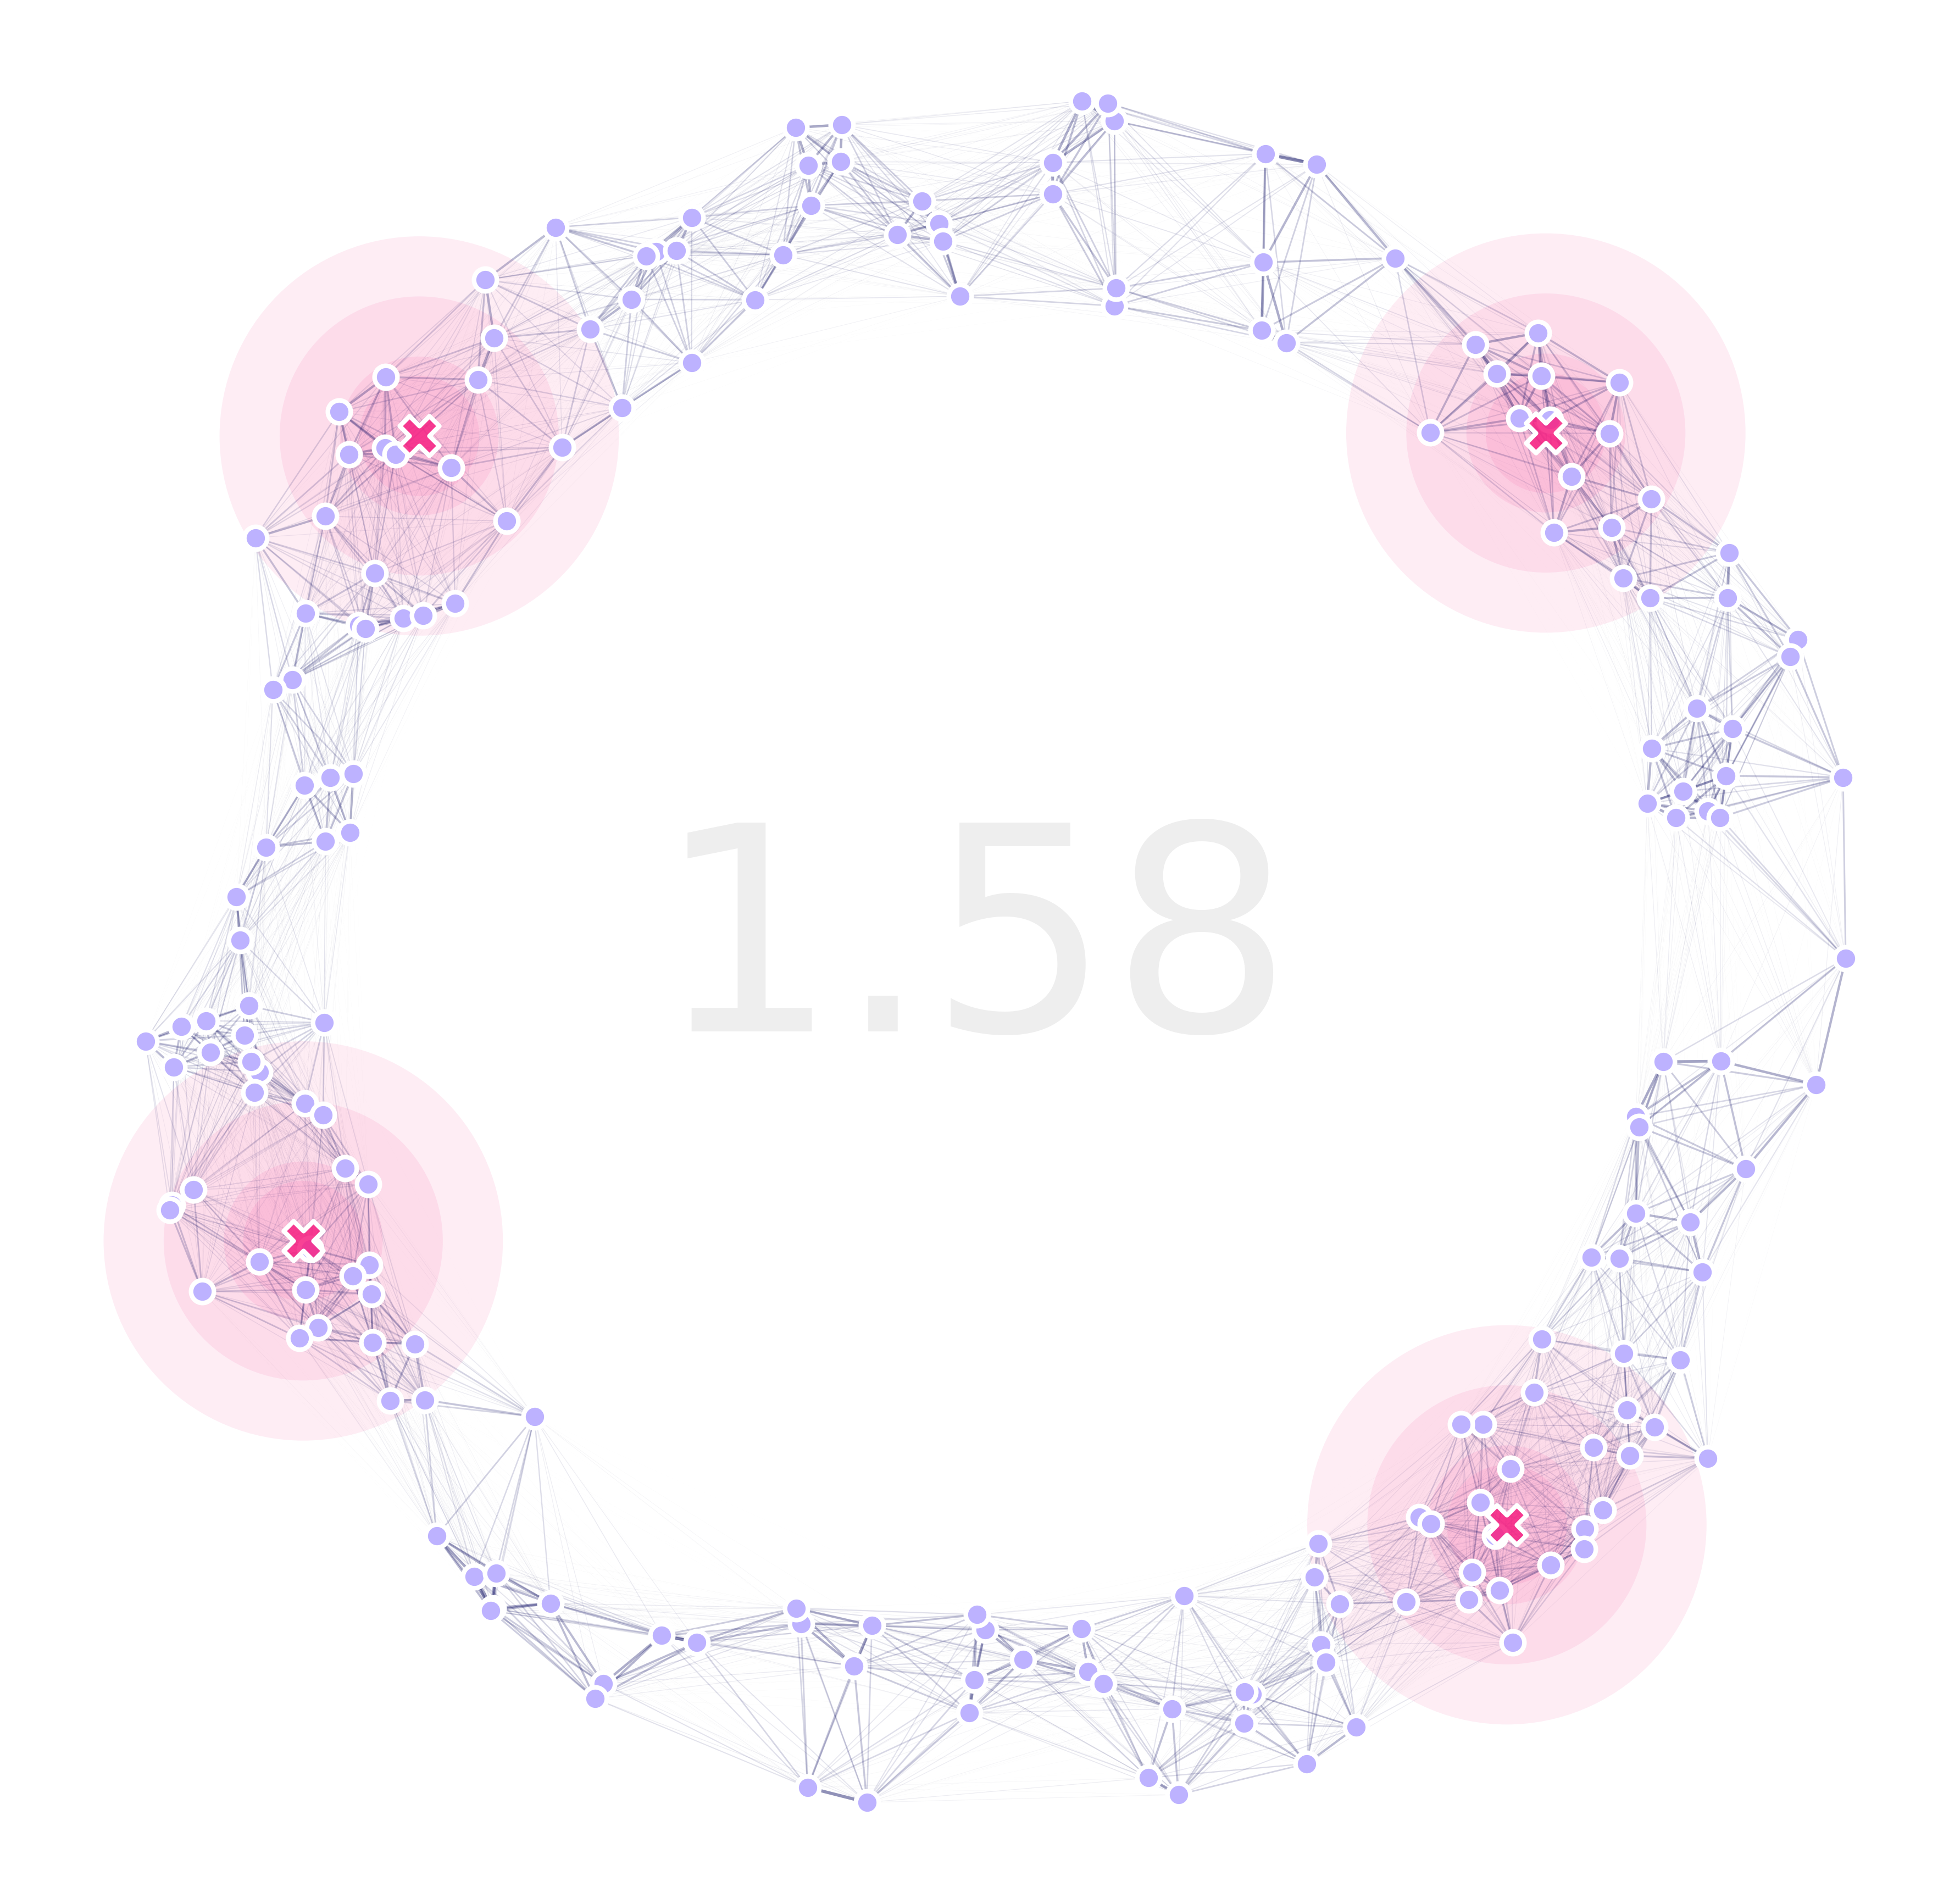
\includegraphics[width=\textwidth]{ga-worst.png}
    \caption{Peor resultado GA}
    \label{fig:ga-worst}
  \end{figure}

\chapter{Interpretación}\label{chap:interpretacion}
\lhead{Capítulo 7. \emph{Interpretación}}
En este capítulo se interpretarán los resultados presentados en el capítulo
anterior para así entender las contribuciones logradas con este trabajo.

Como se puede ver en las Figuras \ref{fig:average-results} y
\ref{fig:percentile}, el PSO logra mejores resultados, en la mayoría de los
casos, que el GA en menos generaciones. Además, aunque al PSO le toma casi el
doble de tiempo en ejecutar las 500 generaciones, los mejores resultados del
PSO son encontrados en 1/5 de las generaciones necesarias para el GA, por lo
que el tiempo de búsqueda fue disminuido con el esfuerzo realizado en el
presente trabajo.

Después de interpretar lo anterior de los resultados obtenidos, se puede decir
que las contribuciones logradas en este trabajo son las siguientes:

\begin{itemize}
  \item Se mejoraron los resultados arrojados por la optimización de trampas
    de mosquitos en el paquete MGSurvE.
  \item Se redujo el tiempo de optimización de trampas para mosquito en el
    paquete MGSurvE.
\end{itemize}

Gracias a estas contribuciones, los recursos asignados para el monitoreo 
variantes de mosquitos en un futuro serán mejor aprovechados y se necesitará
menor cantidad de tiempo para lograr detectar las migraciones de estos
mosquitos en el campo.

Sin embargo, también se puede decir que
el PSO tiene grandes áreas de mejora, como solucionar el problema de los
mínimos locales en el 20\% de los casos. De igual manera, hay oportunidad de
trabajo en la comparación y análisis del algoritmo trabajado, para entender
mejor cómo se comporta con más trampas y diferentes tipos de escenarios y
entornos proporcionados por el paquete MGSurvE.

\chapter{Conclusiones y trabajo futuro}\label{chap:conclusiones}
\lhead{Capítulo 8. \emph{Conclusiones y trabajo futuro}}

  En este capítulo se presentan las conclusiones obtenidas de este trabajo. 
  Se toman en cuenta los trabajos que componen el estado del arte, la solución
  propuesta y los resultados obtenidos de la evaluación de la efectividad del
  algoritmo.

  \section{Conclusiones}

  En la última década se ha visto un incremento en los artículos publicados
  en donde se aplican algoritmos de optimización a distintos campos. Sin
  embargo, las aplicaciones para el control y monitoreo de mosquito son
  mínimas. El trabajo más relevante es MGSurvE, pues es la única herramienta
  enfocada totalmente a la optimización en el ámbito de monitoreo de
  mosquitos.

  La problemática presentada en este trabajo gira en torno a MGSurvE, pues su
  algoritmo de optimización, un GA, no está encontrando las mejores posiciones
  posibles para las trampas de mosquitos, y estos resultados son encontrados
  en etapas tardías de las búsquedas. 

  A partir de esto, se propuso la implementación de un algoritmo PSO para
  reemplazar al GA y mejorar el comportamiento general del paquete MGSurvE.

  Para validar que el algoritmo propuesto cumplía con su propósito, se diseñó
  una metodología basada en la comparación directa de ambos algoritmos, el PSO
  y el GA.
  
  A partir de las métricas generadas de la comparación, se puede concluir que
  el algoritmo PSO propuesto en este trabajo cumple su objetivo de mejorar
  los resultados arrojados por MGSurvE, pues genera mejores posiciones para
  las trampas la mayoría de las veces y lo hace en una menor cantidad de
  generaciones.

  \section{Trabajo futuro}

  Durante el desarrollo y evaluación del algoritmo PSO propuesto en este
  trabajo se encontraron algunas áreas de oportunidad para mejora. Estas
  oportunidades se deben a falta de recursos para el desarrollo. Las posibles
  mejoras futuras son las siguientes:

  \begin{itemize}
    \item Buscar solución al problema de mínimos locales presente en el
      algoritmo PSO.
    \item Graficar el percentil 50 o la media en la Figura
      \ref{fig:percentile} en lugar del promedio para mejorar la visualización
      de los datos.
    \item Realizar una comparación del comportamiento del PSO con diferentes
      cantidades de trampas a optimizar.
  \end{itemize}    
